%%% The main file. It contains definitions of basic parameters and includes all other parts.


%% Settings for two-sided (duplex) printing
\documentclass[10pt,a4paper]{report}
\let\openright=\cleardoublepage

%% Character encoding: usually latin2, cp1250 or utf8:
\usepackage[utf8]{inputenc}

%% It's 2019
\usepackage[default]{droidserif}
\usepackage[T1]{fontenc}

%% Further useful packages (included in most LaTeX distributions)
\usepackage{amsmath}        % extensions for typesetting of math
\usepackage{amsfonts}       % math fonts
\usepackage{graphicx}       % embedding of pictures
\usepackage{tikz}
%\usetikzlibrary{shapes,fit,positioning,snakes,mindmap,trees,decorations.text,arrows.meta}
%\makenomenclature
\usepackage{algorithm,algpseudocode}
\usepackage{booktabs}
\usepackage{mwe}
\usepackage{afterpage}
\usepackage{pgfgantt}
\usepackage{pdflscape}
\usepackage{geometry}
\usepackage{enumitem}
\usepackage{float}
\usepackage{framed}
\usepackage{titlesec}
\usepackage{listings}
\usepackage{xcolor}
\usepackage{longtable}
\usepackage{makecell}
\usepackage[toc,page]{appendix}
\usepackage{multirow}

\lstset{basicstyle=\ttfamily,
	showstringspaces=false,
	commentstyle=\color{red},
	keywordstyle=\color{blue}
}

\usepackage{pdfpages}

\usepackage[textsize=tiny,backgroundcolor=yellow!50, linecolor=black!25]{todonotes}

% links shall be clickable
\usepackage[unicode]{hyperref}   % Must follow all other packages
\usepackage{cleveref} % Must follow all other packages including hyperref

% Definitions of macros (see description inside)

\newcommand{\cool}{\color{green!50!white!80!black}}
\newcommand{\textcool}[1]{{\cool #1}}

\newcommand{\XX}[1]{\textcolor{red}{#1}}
\newcommand{\TT}[1]{\texttt{#1}}
\newcommand{\SC}[1]{{\fontfamily{phv}\selectfont\textsc{#1}}}

% Draw black "slugs" whenever a line overflows, so that we can spot it easily.


% avoid some slugs naturally
\clubpenalty=1000
\widowpenalty=1000
%\hyphenpenalty=100  % turn this on to prevent hyphenation
\emergencystretch=2cm


%%% The field of all real and natural numbers
\newcommand{\R}{\mathbb{R}}
\newcommand{\N}{\mathbb{N}}
\newcommand{\F}{\mathbb{F}}
\newcommand{\Z}{\mathbb{Z}}

\newcommand{\bms}{\begin{enumerate}[label=\bf (M\arabic*)]}
\newcommand{\bwp}{\begin{enumerate}[label=\bf \normalsize  (WP\arabic*), resume=del]}
\newcommand{\eenum}{\end{enumerate}}
\newcommand{\itemm}{\large \item }
\newcommand{\itemwp}{ \normalsize \item }
\newcommand{\deadline}[2]{\small (deadline: \textit{month #1}, duration: \textit{#2 moths})}
\newcommand{\people}[1]{\textit{\small (#1)}}


% move the headings out of gutenberg era
\setcounter{secnumdepth}{4}
\titleformat{\chapter}{\cool\fontsize{24pt}{24pt}\bfseries}{\color{black!25}\thechapter.}{1em}{}
\titleformat{\section}{\cool\fontsize{16pt}{18pt}\bfseries}{\scriptsize\color{black!25}\thesection}{1em}{}
\titleformat{\subsection}{\cool\fontsize{14pt}{16pt}\bfseries}{\scriptsize\color{black!25}\thesubsection}{1em}{}
\titleformat{\subsubsection}{\cool\fontsize{12pt}{14pt}\bfseries}{\scriptsize\color{black!25}\thesubsubsection}{1em}{}

% code floats
\colorlet{shadecolor}{cyan!10}
\makeatletter
\newcommand\floatc@code[2]{{\@fs@cfont #1} #2\par}
\newcommand\fs@code{\def\@fs@cfont{\bfseries}\let\@fs@capt\floatc@code
\def\@fs@pre{}%
\def\@fs@mid{\vspace{-.5ex}\begin{shaded}}%
\def\@fs@post{\vspace{-1em}\end{shaded}}%
\let\@fs@iftopcapt\iftrue}
\makeatother

\floatstyle{code}
\newfloat{listing}{tbp}{lst}
\floatname{listing}{Listing}


\title{\textcool{\bf High Level Assembler Plugin} \\ Project documentation}
\author{Michal Bali, Marcel Hruška, Peter Polák,\\ Adam Šmelko, Lucia Tódová}
\date{Supervisor: Miroslav Kratochvíl \\ \vspace{5mm} Consultant: Slavomír Kučera (Broadcom)}

% Title page and various mandatory informational pages
\begin{document}
\maketitle

%%% A page with automatically generated table of contents of the bachelor thesis

\tableofcontents

%%% Each chapter is kept in a separate file

\chapter{Introduction}

The IBM High Level Assembler Language (HLASM) is still actively used commercially, even though it is a relatively old language. Its roots go back to the 1970s, when IBM made their first mainframes. Since then, the IBM assembler has been revised several times --- the last version (which is the concern of this project) was released in 1992. Although it is hard to believe, a lot of the software that has been written in the language over the years is still actively used and maintained, mainly because of the conservative mainframe users and IBM's vendor lock-in.

Today, HLASM developers are forced to code in archaic terminals directly on the mainframe. Therefore, they spend a lot of time navigating around the code and the environment. For example, solely due to the fact that the user needs to navigate through plenty of terminal screens it takes around a minute just to get to a screen where it is possible to make a change in a file and recompile. For developers, it would be extremely useful to have an IDE plugin that would minimize contact with the mainframe terminal, could analyze the HLASM program, check its validity and make the code clearer by syntax highlighting. 

We introduce such plugin for Visual Studio Code, which is nowadays one of the most popular code editors. It improves HLASM programming experience, so that it can be compared to coding in modern programming languages, by providing instant code validity checks, advanced highlighting, code analysis, and all the functionality that a programmer currently takes for granted when writing code.

Some of the most noteworthy properties and features of the plugin are:
\begin{itemize}
	\item It is capable of interpreting and tracing a large subset of HLASM code-generating instructions
	\item It contains a list of all built-in instructions that is used to validate the generated code
	\item So called \emph{macro tracer} gives a possibility to trace the compilation of HLASM source code step-by-step in a way similar to common debugging.
	\item It implements DAP and LSP protocols, providing interface to be easily integrated into numerous modern code editors
	\item It has been run and tested on over 15 millions lines of real production HLASM code
\end{itemize}
The plugin is available on the Visual Studio Code Marketplace\footnote{\url{https://marketplace.visualstudio.com/items?itemName=broadcomMFD.hlasm-language-support}}

This document serves as an in-depth documentation for anyone who would like to understand the implementation of the project and the reasons behind it. It is advised that the potential contributors to the project read this documentation first.

User documentation is available on the Visual Studio Code marketplace \footnote{\url{https://marketplace.visualstudio.com/items?itemName=broadcomMFD.hlasm-language-support}} or in a markdown file \TT{clients/vscode-hlasmplugin/README.md}. The HLASM plugin project also contains an example workspace that can be used to test out the plugin.


\section{Organisation of this document}
First of all, in~\cref{hlasm}, we briefly explain the basics of HLASM needed to comprehend the workflow of this language. In~\cref{arch}, we provide an overview of the project's architecture, naming the most important components and indicating their relations. Then, we describe these components in separate chapters in further detail. In~\cref{chap:lang_server}, we state the responsibilities of the language server as the communication provider between the extension client and the parsing library. The workspace manager is the entry point to the parsing library used by the language server and it is fully described in~\cref{ws_manager}. The purpose of its sub-components is to handle file management, dependency resolution and parsing. The core of the processing of a HLASM file is implemented inside the analyzer, whose mechanics and implementation details are discussed in~\cref{chap:analyzer}. The project also provides macro tracing through the standard debugging procedure and it is fully explained in~\cref{macro_tracer}.The last mentioned component, detailed in~\cref{extension} is the VSCode extension, which communicates with the language server and provides IDE features to the user. At the end of this document, in~\cref{build}, we provide the instructions on how to build the project.

\part{Project overview}
\chapter{HLASM overview}
\label{hlasm}
Ordinary assembly languages consist solely of ordinary machine instructions. High-level assemblers generally extend them with features commonly found in high-level programming languages, such as control statements similar to \emph{if, while, for} as well as custom callable macros.

IBM High Level Assembler (HLASM) satisfies this definition and adds other features, which will be described in this section.

\section{Syntax}

HLASM syntax is similar to a common assembler, but due to historical reasons it has limitations, like line length limited to 80 characters (as that was the length of a punched card line).

\subsection{Statement}

HLASM program consists of a sequence of \emph{statements}, which are used to produce both compile-time code and run-time code (see \cref{Assembling}). A statement consists of four fields separated by spaces that can be split into more lines using continuations (see \cref{Continuation}). Following are the existing fields:
\begin{itemize}
	\item \textbf{Name field} --- Serves as a place for named constants that are to be used in the code. This field is optional, but, when present, it must start at the begin column of a line.
	
	\item \textbf{Instruction field} --- The only mandatory field, represents the instruction that is executed. It must not begin in the first column, as it would be interpreted as a name field.
	
	\item \textbf{Operands field} --- Field for instruction operands, located immediately after instruction field. Individual operands must be separated by a comma, and, depending on the specific instruction, can be either blank, in a form of an apostrophe separated string, or represented by a sequence of characters.
	
	\item \textbf{Remark field} --- Optional, serves as inline commentary. Located either after the operands field, or, in case the operands are omitted, after the instruction field. 
\end{itemize}

\begin{listing}[t]
	\begin{verbatim}
name    instruction     operands             remark
.NOMOV       AGO     (&WH).L1,.L2,.L3     SEQUENTIAL BRANCH
	\end{verbatim}
	\caption{An example statement.}
	\label{lst:small_example}
\end{listing}

\Cref{lst:small_example} shows an example of a basic statement containing all fields.

\subsection{Continuations}
\label{Continuation}

Individual statements sometimes contain more than 80 characters, which does not agree with the historical line length limitations. Therefore, a special feature called \emph{continuation} exists.

For this purpose the language specification defines four special columns:
\begin{itemize}
	\item \emph{Begin column} (default position: 1)
	
	\item \emph{End column} (default position: 71)
	
	\item \emph{Continuation column} (default position: 72)
	
	\item \emph{Continue column} (default position: 16)
\end{itemize}

The begin column defines where the statements can be started.

The end column determines the position of the end of the line. Anything written to its right does not count as content of the statement, and is rather used as a line sequence number (see \cref{fig01:line}).

The continuation column is used to indicate that the statement continues on the next line. For proper indication, an arbitrary character other than space must be written in this column. The remainder of the statement must then start on the continue column.

An example of an instruction where its last operand exceeded column 72 of the line can be seen in \cref{lst:overflow}.

\begin{listing}[t]
	\begin{verbatim}
    OP1                            REG12,REG07,REG04,REG00,REG01,REG11,Rx
                EG02
	\end{verbatim}
	\caption{Example program that uses the continuation to write a statement longer than 80 characters.}
	\label{lst:overflow}
\end{listing}

Some instructions also support the \emph{extended format} of the operands. This allows the presence of a continuation character even when the contents of a line have not reached the continuation column (see \cref{lst:extended}).

\begin{listing}[t]
	\begin{verbatim}
          AIF   ('&VAR' FIND '~').A,     REMARK1                        x
                ('&VAR'  EQ  'L').B,     REMARK2                        x
                (T'&VAR  EQ  'U').C      REMARK3 
	\end{verbatim}
	\caption{Extended instruction format.}
	\label{lst:extended}
\end{listing}

\begin{figure}
	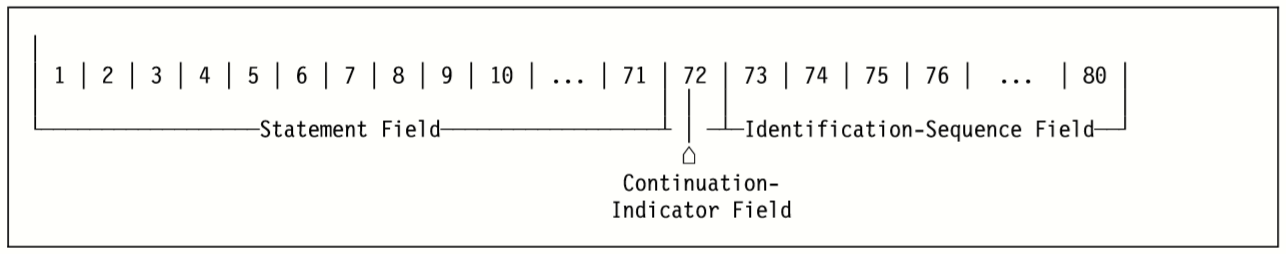
\includegraphics[width=\textwidth]{img/line}
	\caption{Description of line columns (source: \href{https://www-01.ibm.com/servers/resourcelink/svc00100.nsf/pages/zOSV2R3sc264940/$file/asmr1023.pdf}{HLASM Language Reference} ).}
	\label{fig01:line}
\end{figure}


\section{Assembling}
\label{Assembling}

Having briefly outlined the syntax, we now describe the assembly process of HLASM. 

We distinguish two types of processing:

\begin{itemize}
	\item \emph{conditional assembly (CA) processing} --- the main purpose of which is to generate statements for ordinary assembly (see \cref{CA_proc})
	\item \emph{ordinary assembly processing} --- which handles \emph{machine instructions} and \emph{assembler instructions} (see \cref{mach_instr}, \cref{asm_instrs})
\end{itemize}

\subsection{Ordinary assembly}

Ordinary assembly, along with machine and assembler instructions, is responsible for the runtime behavior of the program. It allows the generation of code from both traditional machine instructions and special-purpose assembler instructions. Moreover, it assigns values to \emph{ordinary symbols}.

\subsubsection{Ordinary symbols}
\label{ord_sym}

In HLASM, an \emph{ordinary symbol} is a named run-time constant. It is defined by inputting its name into the name field of a statement along with a special assembler instruction. Each ordinary symbol can only be defined once, and its value is constant. There are two types of ordinary symbols:
 
\begin{itemize}
	\item An \emph{absolute symbol} that simply has an integral value.
	\item A \emph{relocatable symbol} that represents an address in the resulting object code. A relocatable symbol can also be defined by writing the ordinary symbol name into the name field of a statement along with a machine instruction name. The symbol then denotes the address of the given instruction.
\end{itemize}

In addition to symbol value, ordinary symbols also contain a set of \emph{attributes}, the most common ones being \emph{type} and \emph{length}.

\subsubsection{Machine instructions}
\label{mach_instr}

\emph{Machine instructions} represent the actual processor instructions executed during run-time. Similarly to traditional assemblers, they are translated into corresponding opcodes and their operands are processed. However, HLASM also allows expressions to be passed as their operands, which may use ordinary symbols and support integer and address arithmetic.

\subsubsection{Assembler instructions}
\label{asm_instrs}

In addition to machine instructions, HLASM assembler also provides \emph{assembler instructions} (in other systems commonly termed \emph{directives}). They instruct the assembler to make specific actions rather than to assemble opcodes. For example, they generate run-time data constants, create ordinary symbols, organize the resulting object code and generally affect how the assembler operates.

Following are examples of assembler instructions:
\begin{itemize}
	\item \textbf{ICTL} --- Changes values of the previously described line columns (i.e. begin column may begin at column 2 etc.).
	
	\item \textbf{DC}, \textbf{DS} --- Reserves space in object code for data described in operands field and assembles them in place (i.e. assembles float, double, character array, address etc.). These instructions take \emph{data definition} as operands. \Cref{data_def_example} shows examples of data definition.
	
	\item \textbf{EQU} --- Defines ordinary symbols.
	
	\item \textbf{COPY} --- Copies text from a specified file\footnote{Path to the folder of the file is passed to assembler before the start of assembly} (called \emph{copy member}) and pastes it in place of the instruction. It is very similar to the C preprocessor \texttt{\#include} directive.
	
	\item \textbf{CSECT} --- Creates an executable control section, which serves as the start of relative addressing. It is followed by sequence of machine instructions.
\end{itemize}

\begin{figure}[t]
	\begin{verbatim}
CL8'ABC'
    C is type of data definition - array of characters
    L8 specifies length - 8 bytes
    'ABC' is nominal value of the data definition
    CL8'ABC' would assemble 8 bytes, first three of which would be EBCDIC
             representations of letters A, B and C

5AY(A+4,B)
    5 is duplication factor - the nominal value will be repeated 5 times
    A is type - address
    Y is type extension - it modifies the length of the address
    (A+4,B) is nominal value - comma separated expressions that will
            be assembled as addresses
    5AY(A+4,B) would assemble total of 20 bytes, first 2 bytes is value
               of expression A+4, then B and then 4 more copies of the same
	\end{verbatim}
	\caption{Examples of data definition}
	\label{data_def_example}
\end{figure}

\subsubsection{Ordinary symbols resolution}
\label{ordinary_resolution}
All the assembler instructions and ordinary symbols must be resolved before the assembler creates the final object file. However, as the HLASM language supports forward declaration of ordinary symbols, the assembly may be quite complicated. Consider an example in \cref{lst:ordinary_assembly}. When the instruction on line 1 is seen for the first time, it is impossible to determine its length, because the symbol \verb|LEN| is not defined yet \footnote{Character L with an expression in parentheses in DS operand of type C specifies how many bytes should be reserved in the program.}. The same applies to the length of the instruction on the second line. Furthermore, it is also impossible to determine the exact value of relocatable symbols \verb|ADDR| and \verb|HERE| because of the unknown length of the preceding instructions.

\begin{listing}[t]
	\begin{Verbatim}[numbers=left]
           DS    CL(LEN)
ADDR       DS    CL(SIZE)

HERE       DS    0H
LEN        EQU   HERE-ADDR
SIZE       EQU   1
	\end{Verbatim}
	\caption{A sample program that shows that symbols can be used prior to their definition.}
	\label{lst:ordinary_assembly}
\end{listing}


In the next step, \verb|LEN| is defined. However, it cannot be evaluated, because the subtraction of addresses \verb|ADDR| and \verb|HERE| is dependent on the unknown length of instruction on second line and therefore on the symbol \verb|SIZE|. The whole program is resolved only when the assembly reaches the last line, which defines the length of instruction \verb|02|. Afterwards, it is possible to resolve \verb|LEN| and finally the length of instruction \verb|01|.

The dependency graph created from these principles can be arbitrarily deep and complicated, however it must not contain cycles (a symbol must not be transitively dependent on itself).

\subsection{Object file layout}

The product of ordinary assembly is an object file. Let us briefly describe its layout.

\subsubsection{Sections}

An object file consists of so-called \emph{sections}. They are user-defined (by instructions CSECT, DSECT, \ldots) and can be of different kinds, each with various properties. Absolute positions of sections within the object file are undefined --- they are determined automatically after the compilation. This also implies that all relocatable symbols are only defined relatively to the section that contains them.

\subsubsection{Location counter}
\label{loctr}

Any time a machine instruction is encountered, its opcode is outputted to the \emph{next available address}. Each section has a structure pointing to this address --- a so-called \emph{location counter}.

The user may define more location counters and then arbitrarily switch between them to state the next address for code generation. Therefore, at all times, there is one and only one location counter active, which defines where the next machine instruction will be generated.

At the end of assembly, all code denoted by location counters is assembled in a well-defined order, and so the absolute position of all relocatable symbols within their section is known.

The value of the location counter can be arbitrarily changed by the ORG instruction. It can be moved backwards or forwards (with restriction of counter underflow) to set the next address. This means that user can generate some code, move counter backwards and overwrite it. Then the ORG instruction can be used to set location counter to the next available untouched address to continue in object creation.

\subsection{Conditional assembly}
\label{CA_proc}

Conditional assembly is another feature provided by HLASM. It is essentially a macro-language built on top of a traditional assembler.

User may use conditional assembly instructions to either define \emph{variable symbols}, which can be used in any statement to alter its meaning, or to define \emph{macros} --- reusable pieces of code with parameters. Based on these instructions, conditional assembly then alters the textual representation of the source code and selects which lines will be processed next.

\subsubsection{Variable symbols}
\label{var_sym}`
Variable symbols serve as compile-time variables. Statements that contain them are called \emph{model statements}.

During conditional assembly, variable symbols are substituted for their value to create a statement processable by ordinary assembly. For example, a user can write a variable symbol in the operation field and generate any instruction that can be a result of a substitution.

Variable symbols also have notion of their type --- they can be defined either as integer, boolean or string. CA instructions gather this information for different sorts of conditional branching.

\subsubsection{CA instructions}
\label{ca_instr}

CA instructions are not assembled into object code. They are used to select which instructions will be processed by the assembler next.

One example of their capabilities is conditional and unconditional branching. As HLASM provides a variety of built-in binary or unary operations on variable symbols, complex conditional expressions can be created. This is important in HLASM, as the user can alter the flow of instructions that will be assembled into an executable program.

Another subset of CA instructions operates on variable symbols. These can be used to define variable symbols locally or globally, assign or update their values.

\subsubsection{Macros}

A \emph{macro} is a structure consisting of a \emph{name}, \emph{input parameters} and a \emph{body}, which is a sequence of statements. When a macro is called in a HLASM program, each statement in its body is executed. Both nested and recursive calls of macros are allowed. Macro body can also contain CA instructions, or even a sequence of instructions generating another macro definition. With the help of variable symbols, HLASM has the power to create custom, task specific macros.

\vspace{5mm}

An example of a simple HLASM program with the description of its statements is shown in \cref{lst:example}.

On lines \verb|01-04|, we see a \emph{macro definition}. It is defined with name \verb|GEN_LABEL|, variable \verb|NAME| and contains one instruction in its body, which assigns the current address to the label in \verb|NAME|.

On line \verb|06|, the \emph{copy instruction} is used, which includes the contents of the \verb|REGS| file.

Line \verb|08| establishes a start of an executable section \verb|TEST|. 

On line \verb|09|, an integer value is assigned to a variable symbol \verb|VAR|. The value is the length attribute of previously non-defined constant \verb|DOUBLE|. The assembler looks for the definition of the constant to properly evaluate the conditional assembly expression. In the next line, there is a CA branching instruction \verb|AIF|. If value of \verb|VAR| equals 4, all the text between \verb|AIF| and \verb|.END| is completely skipped and assembling continues on line \verb|18|, where the branching symbol \verb|.END| is located.

Lines \verb|12-13| show examples of machine instructions that are directly assembled into object code. Lines \verb|11| and \verb|14| contain examples of a macro call.

On line \verb|15|, the constant \verb|LEN| is assigned the difference of two addresses, which results in absolute ordinary symbol. This value is next used to generate character data.

Instruction \verb|DC| on line \verb|17| creates value of type double and assigns its address to the ordinary symbol \verb|DOUBLE|. This constant also holds information about length, type and other attributes of the data.  

\verb|ANOP| is an empty assembler action which defines the \verb|.END| symbol and line \verb|19| ends the assembling of the program. 

%\let\oldv\verbatim
%\let\oldendv\endverbatim

%\def\verbatim{\par\hspace{1cm}\setbox0\vbox\bgroup\oldv}
%\def\endverbatim{\oldendv\egroup\fboxsep0pt \colorbox[gray]{0.8}{\usebox0}\par}

\begin{listing}[t]
    \begin{verbatim}
name        operation   operands
    \end{verbatim}
	\begin{Verbatim}[numbers=left]
            MACRO                   
&NAME       GEN_LABEL
&NAME       EQU         *
            MEND
        
            COPY        REGS
        
TEST        CSECT
&VAR        SETA        L'DOUBLE
            AIF         (&VAR EQ 4).END
LBL1        GEN_LABEL
            LR          3,2
            L           8
LBL2        GEN_LABEL
LEN         EQU         LBL2-LBL1
            DC          (LEN)C'HELLO'
DOUBLE      DC          H'-3.729'
.END        ANOP
            END
	\end{Verbatim} 
	\caption{An example of an artificial HLASM program.}
	\label{lst:example}
\end{listing}

\vspace{5mm}

Although CA processing may act like text preprocessing, it is still interlinked with ordinary processing. CA has mechanics that allow the assembler to gather information about statements that are printed during the processing. It can also access values created in ordinary assembly and use them in conditional branching, and is able to lookup constants that are not yet defined prior to the currently processed statement. During ordinary assembly, names of these instructions can also be aliased.

To sum up, CA processing has variables for storing values during the compilation and CA instructions for conditional branching. Hence, it is Turing-complete while still evaluated during compile-time.

\section{HLASM source structure}

The file that generates the object code is called an \emph{open-code} file. It is the entry file of the HLASM compiler. Each open-code file can have in-file dependencies, specifically:
\begin{itemize}
	\item External Macro definitions
	\item Copy members
\end{itemize}
These are not treated as open-code files because they do not directly generate object code. Rather, they serve as statement sequences that are included in specific places of open-code and provide specific meaning.



\chapter{Architecture overview}
\label{arch}

\begin{figure}
	\centering
	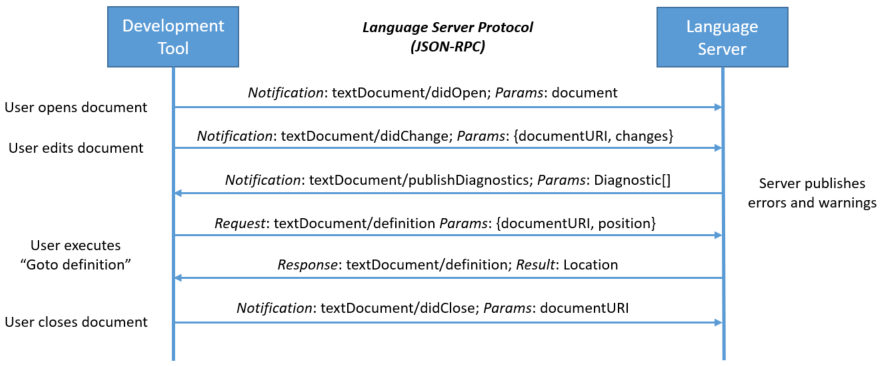
\includegraphics[width=\textwidth]{img/language-server-sequence}
	\caption[LSP session example.]{LSP session example. (source: \url{https://microsoft.github.io/language-server-protocol/overview} )}
	\label{fig04:LSP}
\end{figure}

\begin{figure}
	\centering
	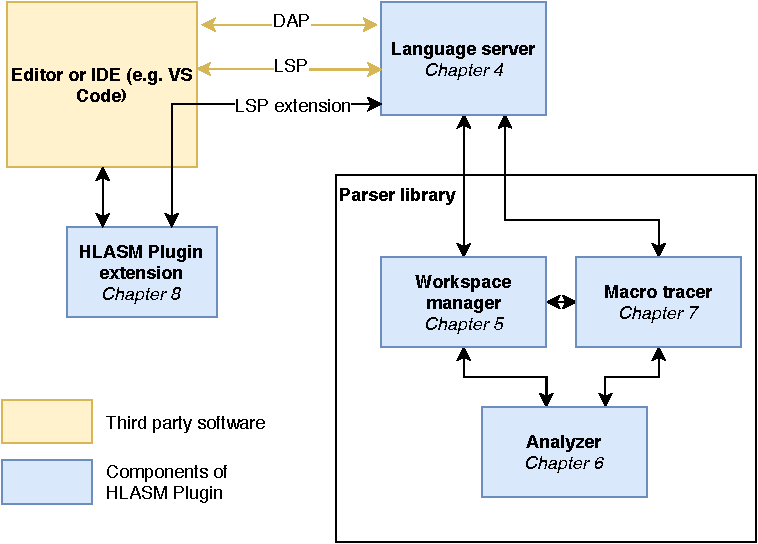
\includegraphics[width=\textwidth]{img/hlasm_architecture}
	\caption{The architecture of HLASM Plugin}
	
	\label{fig04:arch}
\end{figure}

The architecture is based on the way modern code editors and IDEs are extended to support additional languages. We chose to implement Language Server Protocol \footnote{\url{https://microsoft.github.io/language-server-protocol/}} (LSP), which is supported by a majority of contemporary editors.

In LSP, the two parties that communicate are called a \emph{client} and a \emph{language server}. A simple example is displayed in \cref{fig04:LSP} The client runs as a part of an editor. The language server may be a standalone application that is connected to the client by a pipe or TCP. All language-specific user actions (for example the Go to definition command) are transformed into standard LSP messages and are sent to the language server. The language server then analyzes the source code and sends back a response, which is then interpreted and presented to the user in editor-specific way. This architecture makes possible to only have one LSP client implementation for each code editor, which may be reused by all programming languages. And vice versa, every language server may be easily used by any editor that has an implementation of the LSP client.

To add support for HLASM, we have implemented the LSP language server and written a lightweight extension to an editor, which uses an already existing implementation of the LSP client. To implement source code highlighting, we had to extend the protocol with a new notification. This notification is used for transferring information from the language server to the VS Code client, which is extended to highlight code in editor based on the incoming custom notifications.

In this chapter, we further decompose the project into smaller components and describe their relations. The two main components are the parser library and the language server --- an executable application that uses the parser library. An overview of the architecture is pictured in \cref{fig04:arch}. The architecture of whole project is shown in \cref{all_arch}

\section{Language server description}

The responsibility of the language server component is to maintain the LSP session, convert incoming JSON messages and use the parser library to execute them. The functionality includes:
\begin{itemize}
    \item reading LSP messages from either a standard input or TCP and writing responses
    \item parsing JSON RPC to C++ structures, so they can be further used
    \item serializing C++ structures into JSON, so it can be sent back to the client
    \item implementing asynchronous request handling: e.g. when a user makes several consecutive changes to a source code, parsing on every change is not needed
\end{itemize}

\section{Parser library description}

Parser library is the core of the project --- it encapsulates the analyzer, which provides all parsing capabilities, and workspace manager, which keeps track of open files in the editor and manages their dependencies. It has to keep the representation of workspaces and files in the parser library exactly the same as the user sees in the editor. It also starts the analyzer when needed, manages workspace configuration and provides external macro and copy libraries to analyzer.

\subsection{Parser library API}
The parser library API is based on LSP --- every relevant request and notification has a corresponding method in the parsing library.

Firstly, the API implements the LSP notifications that ensure the editor state synchronization. Apart from working with individual files, the LSP also supports workspaces. A workspace is basically just a folder that contains related source codes. The LSP also supports working with multiple workspaces at the same time. We use it when searching for dependencies of HLASM source codes (macros, and copy files).

The parser library needs to have the exact contents of all files in open workspaces. To achieve that, there is a file watcher running in the LSP client that notifies the server when any of the HLASM source files is changed outside of editor. For example, when a user deletes an external macro file, the parser library should react by reporting that it cannot find the macro.

Following is the list of necessary editor state synchronization notifications:
\begin{itemize}
	\item Text synchronization notifications (didOpen, didChange, didClose) that inform the library about files that are currently open in the editor and their exact contents.
	\item DidChangeWorkspaceFolders notification that informs the library when a workspace has been opened or closed.
	\item DidChangeWatchedFiles notification
\end{itemize}

Secondly, the API implements the requests and notifications that provide the parsing results, specifically:
\begin{itemize}
	\item publishDiagnostics notification. A diagnostic is used to indicate a problem with source files, such as a compiler error or a warning. The parser library provides a callback to let the language server know that diagnostics have changed.
	\item Callback for highlighting information provision.
	\item Language feature requests (definition, references, hover, completion), which provide information needed for proper reaction of the editor on user actions.
\end{itemize}

\subsection{Analyzer}

The analyzer is able to process a single HLASM file. The processing includes:
\begin{itemize}
 \item recognition of statements and their parts (lexing and parsing)
 \item interpretation of instructions that should be executed in compile time
 \item a check whether the HLASM source code is well-formed
 \item reporting of problems with the source by producing LSP diagnostics
 \item providing highlighting and LSP information
\end{itemize}

A HLASM file may have dependencies --- other files that define macros or files brought in by the COPY instruction. The dependencies are only discovered during the processing of files, so it is not possible to provide the files beforehand. The analyzer gets a callback that would find a file with specified name, parse its contents and return it as list of parsed statements. 

To sum up, the analyzer has a pretty simple API: it takes the contents of a source file by common string and a callback that can parse external files with specified name. It provides a list of diagnostics linked to the file, highlighting, list of symbol definitions, etc.

\section{Client-side VS Code extension}
\label{arch:client}

The VS Code extension component ensures seamless integration with the editor. Its functions are:

\begin{itemize}
	\item to start the HLASM language server and the LSP client that comes with VS Code, and to create a connection between them.
	\item to implement extension of the LSP protocol for enabling server-side highlighting. The extended client parses the information from the server and uses VS Code API to actually color the text in the editor.
	\item to implement continuation handling --- when the user types something in front of the continuation character, it should stay in place.
\end{itemize}


\section{Macro tracer}
\label{arch:macro}
The macro tracer enables the user to trace the compilation of HLASM source code in a way similar to common debugging. This is the reason why we chose to implement the Debug Adapter Protocol \footnote{\url{https://microsoft.github.io/debug-adapter-protocol/}} (DAP). It is very similar to LSP, so most of the code implementing LSP in the language server component may be reused for both protocols.

The language server component communicates with the macro tracer component in the parser library. Its API mirrors the requests and events of DAP.

Following are the most important DAP features implemented by macro tracer:

\begin{itemize}
	\item launch, continue, next, stepIn and disconnect requests, which allow the user to control the flow of the compilation
	\item SetBreakpoints, which transfers the information about breakpoints that the user has placed in the code
	\item Threads, StackTrace, Scopes and Variables requests to allow the DAP client to retrieve information about the current processing stack (stack of nested macros and copy instructions), available variable symbols and their values
	\item stopped, exited and terminated events to let the DAP client know about state of traced source code
\end{itemize}

The macro tracer communicates with the workspace manager to retrieve the content of the traced files. Afterwards, it starts analyzing the source file in a separate thread and gets callbacks from the analyzer before each statement is processed. In the callback, the tracer puts the thread to sleep and waits for user interaction. During this time, it is possible to retrieve all variable and stack information from the processing to display it to the user.


\part{Component description}
\chapter{Language server}
\label{chap:lang_server}
The purpose of the Language server is to implement the Language Server Protocol (LSP) and the Debug Adapter Protocol (DAP) and to provide access to the parser library by using them. It has to deserialize and serialize LSP and DAP messages, extract parameters of particular methods and then serve the requests by invoking functionality of parser library.

\section{Language Server Protocol}
Language Server Protocol is used to extend code editors with support for additional programming languages. LSP defines 2 communicating entities: a client and a server. The LSP client is editor-specific and wraps interaction with the user. The LSP server is language-specific and provides information about the source code.

The main purpose of the LSP is to allow the language server to provide language-specific response to various user interactions with the code editor. Messages that flow through LSP can be divided into three categories:

\begin{itemize}
	\item \textbf{Parsing results presentation} Messages from the first category allow the language server to send results of source code analysis to the LSP client. The editor is then able to show them to the user. For example, when the user clicks on a symbol in HLASM code and then uses the `Go to definition' function, the LSP client sends a request to the language server with the name of currently open file and current location in the file. The server is then expected to send back the location of the definition, so the editor can present it to the user (e.g. the editor moves the caret to the definition location). List of all such messages is in \cref{lsp_parse_results}.

	\item \textbf{Editor state and file content synchronization} Messages from the second category flow mainly from the client to the server and ensure that the server has enough information to correctly analyze source code. List of all such messages can be found in \cref{lsp_text_sync_methods}.
	
	\item \textbf{LSP initialization and finalization} Lastly, there are several messages that handle protocol initialization and finalization.
\end{itemize}


\begin{table}
	\centering
	\begin{tabular}{ll}
		
		\toprule
		Message & Description \\ \midrule
		& \multirow{3}{9cm}{The client sends a position in an open file. The server responds with a position of a definition of a symbol at that position.} \\
		textDocument/definition &  \\
		& \\
		& \\
		& \multirow{3}{9cm}{The client sends a position in an open file. If there is a symbol, the server responds with a list of positions where the symbol is used.}\\
		textDocument/references & \\
		& \\
		& \\
		& \multirow{3}{9cm}{The client sends a position in an open file where the user is pointing with the cursor. The server responds with a string to be shown in a tooltip window.}\\
		textDocument/hover & \\
		& \\
		& \\
		& \multirow{3}{9cm}{The client sends a position in an open file and how a completion box was triggered (i.e. with what key, automatically/manually). The server responds with a list of strings suggested for completion at the position.}\\
		textDocument/completion & \\
		& \\
		& \\
		& \\
		\multirow{3}{4cm}{textDocument/\\publishDiagnostics} & \multirow{3}{9cm}{The server sends diagnostics to the client. A diagnostic represents a problem with the source code, e.g. compilation errors and warnings.}\\
		 & \\
		& \\ \bottomrule
	\end{tabular}
	
	\caption{List of all results-presenting messages}
	\label{lsp_parse_results}
\end{table}

\begin{table}
	\centering
	\begin{tabular}{ll}
		
		\toprule
		Message & Description \\ \midrule
		textDocument/didOpen & \multirow{3}{8.5cm}{The server is notified whenever the user opens a file, changes contents of an already open file or closes a file in the editor.} \\
		textDocument/didChange & \\
		textDocument/didClose & \\
		& \\
		 &\multirow{4}{8.5cm}{The client notifies the server when a watched file is changed outside of the editor. Watched files selector is defined when the client is started (in the extension component).} \\
		workspace/ & \\
		didChangeWatchedFiles& \\
		& \\
		& \\
		workspace/ & \multirow{2}{8.5cm}{The client notifies the server that the user has opened or closed a workspace.} \\
		didChangeWorkspaceFolders & \\ \bottomrule
	\end{tabular}
	
	\caption{List of all implemented editor state and text synchronization messages}
	\label{lsp_text_sync_methods}
\end{table}


LSP is based on JSON RPC\footnote{\url{https://www.jsonrpc.org/specification}}. There are two types of interaction in JSON RPC: requests and notifications. Both of them carry the information to invoke a method on the recipient side ---  name of the method and its arguments. The difference between the two is that each request requires a response containing the result of the method, whereas the notifications do not.

The LSP uses the JSON RPC specification and further specifies how messages are transferred and defines methods, their arguments, responses and semantics. A raw message sent from the client to the server is shown in \cref{hover_message}.

\begin{listing}
	\begin{verbatim}
Content-Length: 123\r\n
\r\n
{"jsonrpc":"2.0","method":"textDocument/didClose","params":{"textDocument":
{"uri":"file:/c%3A/Users/admin/Documents/source.hlasm"}}}
	\end{verbatim}
	\caption{An example of a message sent from the client to the server.}
	\label{hover_message}
\end{listing}

The raw messages have HTTP-like headers. The only mandatory header is \TT{Content-Length}, which tells the recipient the length of the following message. The JSON itself is sent after the header.

Inside the JSON, there is a name of the method to be invoked and parameters to pass to the method. In this case, the client is sending a notification that file ``C:/Users/admin/Documents/source.hlasm'' was closed in the editor by the user. As it is a notification, there must not be any response.

On top of this basic protocol, LSP defines methods and their semantics to cover common functionality that users expect when programming in an editor. List of all methods implemented in the language server can be found in \cref{LSP_methods}.

\section{DAP}
Debug Adapter Protocol is used to extend code editors with debugging support for additional programming languages. We use it to provide the user with the ability to trace how the HLASM compiler processes source code step by step. The user can see the values of compile-time variables and follow the expansion of macros in debug-like experience.

The communication in DAP is between an editor or an IDE and a debugger. The editor notifies the debugger about the user actions, e.g. when a breakpoint is set or when the user uses step in/step over buttons. The debugger informs the editor about the state of the debugged application, for example when the debugger stopped because it hit a breakpoint. While it is stopped, the debugger sends information about program stack, variables valid in current debugger scope and its values.

DAP is very similar to LSP. Although the ideas behind DAP are nearly the same, DAP is not based on the JSON RPC. Instead, DAP specifies its own implementation of remote procedure call, still using JSON as the basic carrier of the messages. DAP has requests and events --- requests always go from the client to the server and require response. Events are the same as the notifications from JSON RPC that are sent from the server to the client. The similarity allows our language server component to share a lot of code between the implementations of the protocols.

\section{Language server overview}
The architecture of the Language server component is illustrated in \cref{lang_server_arch}. It communicates on the standard input/output via LSP with the LSP client and listens on a TCP port to provide DAP support for the macro tracer. The TCP communication is wrapped by class \TT{tcp\_handler}, which abstracts from the complexity of communicating through TCP/IP.


\begin{figure}
	\centering
	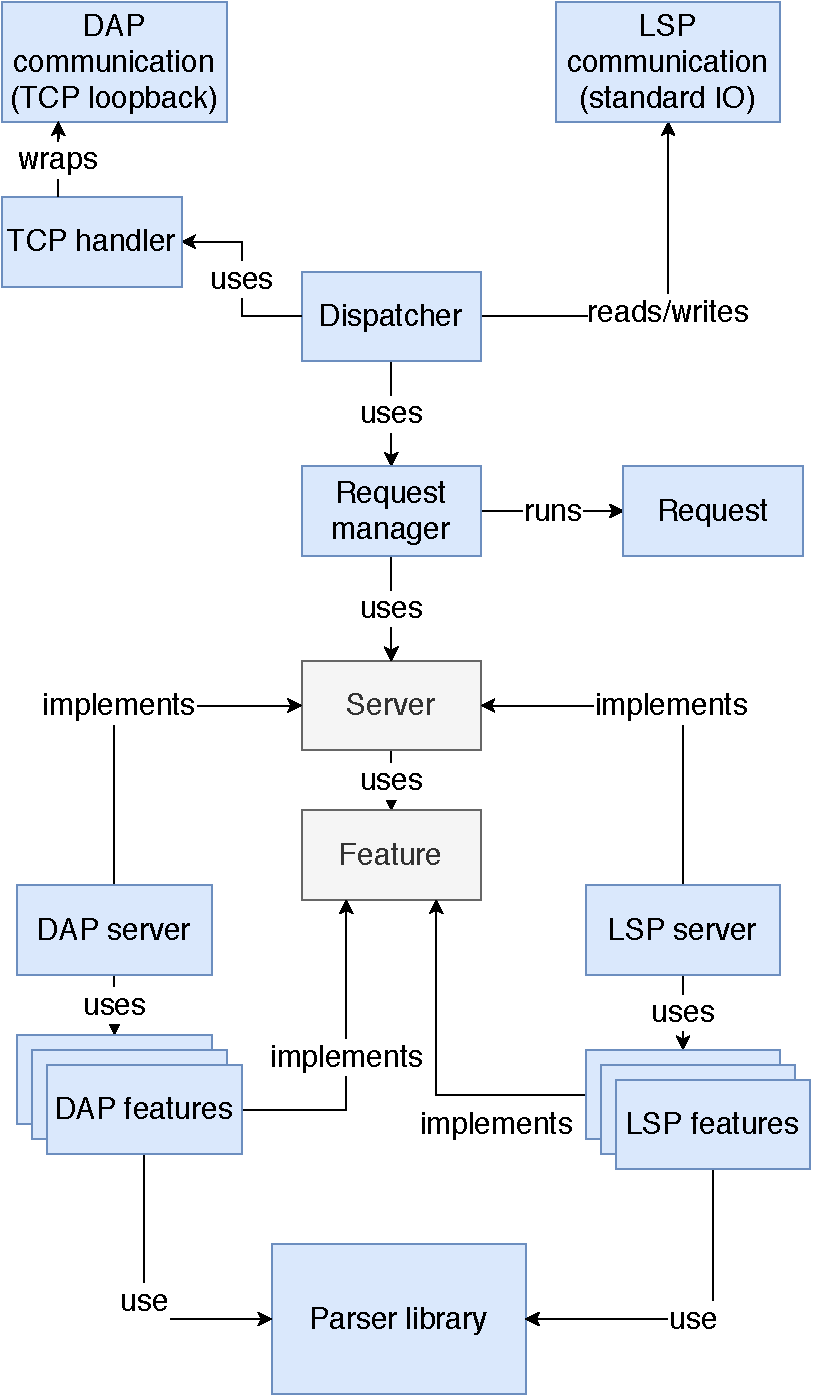
\includegraphics[width=11cm]{img/lang_server}
	\caption{Architecture of language server.}
	\label{lang_server_arch}
\end{figure}


The main purpose of the class \TT{dispatcher} is to provide abstraction for the lowest level communication, which is shared by LSP and DAP. It reads iostream to parse messages using the JSON for Modern C++ library (see \cref{3rd_party}) and stores them in the \TT{request\_manager} as \TT{requests}.

A \TT{request} encapsulates one message that came from the client and is basically represented only by raw (but parsed) JSON.

\TT{request\_manager} stores \TT{requests} in a queue and runs a worker thread that serves the requests one by one. As there is only one instance of request manager running in the language server, it serializes requests from DAP and LSP (which come asynchronously from separate sources) into one queue.

\TT{server} is an abstract class that implements protocol behavior that is common for both DAP and LSP --- it basically implements Remote Procedure Call. Actual handling of LSP and DAP requests is implemented in \TT{features}. Each \TT{feature} contains implementation of several protocol requests or notifications. The features unwrap the arguments from JSON and call corresponding parser library methods.

There are two implementations of the abstract \TT{server} class: \TT{lsp\_server} and \TT{dap\_server}. They both implement the initialization and finalization of protocol communication, which is a bit different for both protocols and both use features to serve protocol requests.

\section{Example: hover request handling}

The \cref{hover_sequence} shows handling of the hover request in the language server. The hover request is sent from the LSP client to the \TT{lsp\_server} when the user hovers over the text of a file. The hover request contains location of the mouse cursor in text, i.e. the name of the file, the number of line and column where the cursor is. The LSP client then expects a response containing a string (possibly written in markdown language) to be shown in a tooltip box.

The whole process begins with reading from the standard input by the LSP instance of the \TT{dispatcher}. It first reads the header of the message, which contains the information about the length of the following JSON. Then it reads the JSON itself and deserializes it using the JSON for Modern C++ library (see \cref{3rd_party}). All other components of the language server work only with the parsed representation of the message. The \TT{dispatcher} adds the message to the \TT{request\_manager} and returns to reading the next message from the standard input.

The request in the \TT{request\_manager} either waits in a queue to be processed, or, if the queue was empty, the worker thread is woken up from sleep using conditional variable. The worker then passes the JSON to the \TT{lsp\_server}, which looks at the name of the method written in the message and calls the method ``hover'' from the language feature.

The hover method unpacks the actual arguments from JSON and converts any URIs to paths using the cpp-netlib URI library. Then, it calls the hover method from the parser library, which returns a string to be shown in the tooltip next to the hovering mouse. The language feature then wraps the return value back in JSON and calls the \TT{respond} method of its \TT{response\_provider} implemented by the \TT{lsp\_server}.

The \TT{lsp\_server} wraps JSON arguments into a LSP response and uses the \SC{send message provider} implemented by \SC{Dispatcher} to send it to the LSP client. The Dispatcher serializes the JSON, adds the header with the length of the JSON and writes the message to a standard output. Finally, all methods return and the worker thread in request manager looks for another request. If there is none, it goes to sleep.

%******************** IO HANDLING *************************
\sectionSrc{I/O handling}
{language\_server/src/main.cpp,language\_server/src/dispatcher.h,language\_server/src/dap/tcp\_handler.h}

The purpose of the \TT{dispatcher} is to abstract from the complexity of working with raw strings and streams. It executes an infinite loop in which it reads messages from \TT{std::iostream} and adds them to the request manager as parsed JSON objects. At the same time, it is able to write responses in the correct format.

The language server communicates with the LSP client on a standard input and output, so we simply use the \SC{dispatcher} with the standard \TT{std::cin} and \TT{std::cout} objects to communicate with the LSP client.

The DAP communicates using TCP/IP, which is less straightforward. Before the VS Code extension starts the language server, it finds a free TCP port and passes it as an argument to the language server executable. The \TT{TCP handler} then starts listening on that port. Once the user wants to start the macro tracer, the DAP client connects to the port on localhost. The \TT{tcp\_handler} accepts the TCP client and creates a \TT{dispatcher} and a \TT{dap\_server}. Once the DAP communication ends, both the \TT{dispatcher} and the \TT{dap\_server} are destroyed and the \TT{tcp\_handler} starts listening again for the next DAP session. Thanks to the ASIO library (see \cref{3rd_party}) implementation of the \TT{std::iostream} interface, the \TT{dispatcher} is able to completely abstract from the fact that it is communicating through TCP and not through the standard IO.

\afterpage{
\begin{landscape}
	\begin{figure}
		\centering
		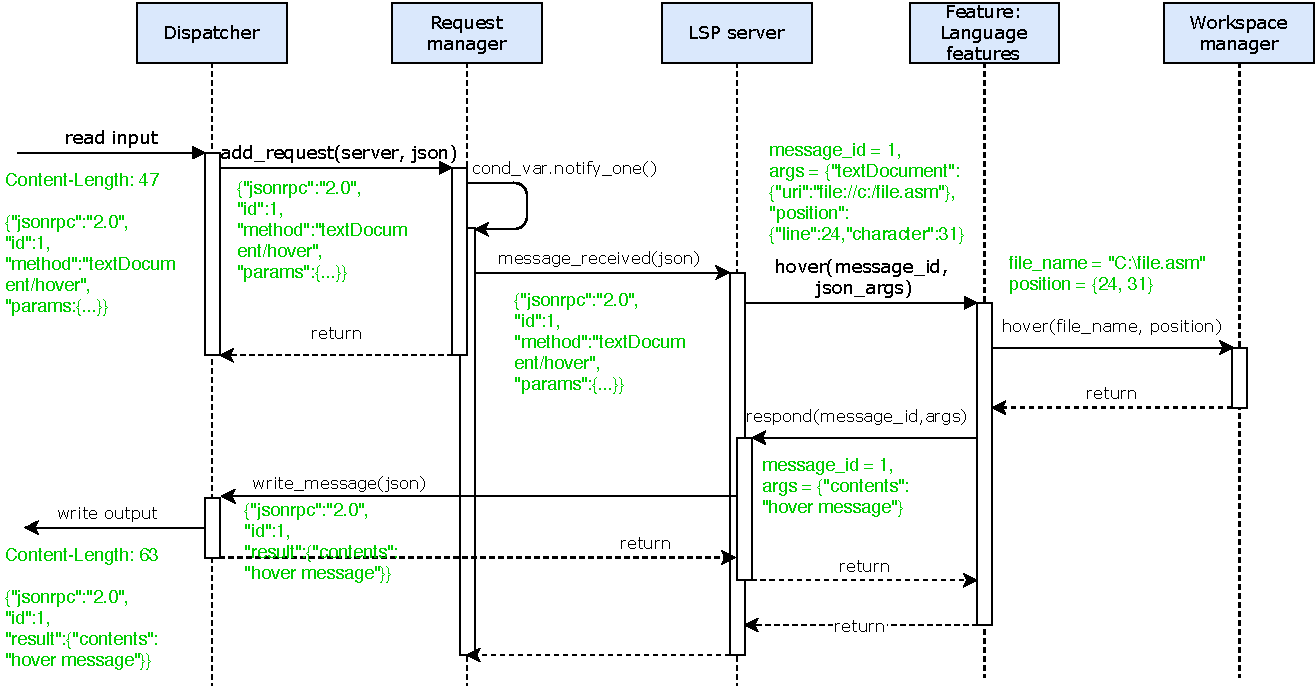
\includegraphics[width=21cm]{img/hover_sequence}
		\caption{A sequence diagram showing the processing of the textDocument/hover request in the language server. The green text represents an example of data passed in the arguments.}
		\label{hover_sequence}
	\end{figure}
\end{landscape}
}

%******************** SERVERS *************************
\sectionSrc{LSP and DAP Server}
{language\_server/src/server.h,language\_server/src/feature.h,language\_server/src/lsp/lsp\_server.h,language\_server/src/dap/dap\_server.h,language\_server/src/dap/dap\_feature.h}
The servers are able to process incoming LSP and DAP requests. They get the messages in a form of already parsed JSONs. Then they extract the name of the requested method with its parameters from the message and call the corresponding method with the parameters encoded as JSON.

There are two server implementations: \TT{lsp\_server} and \TT{dap\_server}. Both inherit from an abstract class called \TT{server}. They implement protocol-specific processing of messages --- although the protocols are quite similar, each protocol has different initialization and finalization, different message format, etc.

The implementation of servers' functionality is divided into features. Each feature implements several LSP or DAP methods by unpacking the arguments of the respective method and calling corresponding parser library function. During initialization, each feature adds its methods to the server's list of implemented methods. The \TT{lsp\_server} uses three features:
\begin{itemize}
	\item \emph{Text synchronization feature}, which handles the notifications about the state of open files in the editor.
	\item \emph{Workspace folders feature}, which handles the notifications about adding and removing workspaces.
	\item \emph{Language feature}, which handles requests about HLASM code information.
\end{itemize}
The \cref{LSP_methods} shows the list of all implemented LSP methods and the classes where the implementations lie.

\begin{table}
	\centering
	\begin{tabular}{ll}
		\toprule
		\textbf{LSP Method name}            & \textbf{Component}                              \\ \midrule
		initialize                          & \multirow{4}{7cm}{LSP server \\ \srcstyle{language\_server/src/lsp/lsp\_server.h}}                   \\
		shutdown                            &                                                 \\
		exit                                &                                                 \\
		textDocument/publishDiagnostics     &                                                 \\ \midrule
		textDocument/didOpen                & \multirow{4}{7cm}{Text synchronization feature \srcstyle{language\_server/src/lsp/feature\_text\_synchronization.h}} \\
		textDocument/didChange              &                                                 \\
		textDocument/didClose               &                                                 \\
		textDocument/semanticHighlighting   &                                                 \\ \midrule
		workspace/didChangeWorkspaceFolders & \multirow{2}{7cm}{Workspace folders feature \srcstyle{language\_server/src/lsp/feature\_workspace\_folders.h}}    \\
		workspace/didChangeWatchedFiles     &                                                 \\ \midrule
		textDocument/definition             & \multirow{4}{7cm}{Language feature \srcstyle{language\_server/src/lsp/feature\_language\_features.h}}             \\
		textDocument/references             &                                                 \\
		textDocument/hover                  &                                                 \\
		textDocument/completion             &                                                 \\ \bottomrule
	\end{tabular}
	\caption{The list of all implemented LSP methods and the classes where they are implemented}
	\label{LSP_methods}
\end{table}

The DAP server uses only one feature --- the Launch feature, which handles stepping through the code and retrieving information about both variables and stack trace. The table \cref{DAP_methods} shows the list of all implemented DAP methods.

\begin{table}
	\centering
	\begin{tabular}{ll}
		\toprule
		\textbf{DAP Method name} & \textbf{Component}                 \\ \midrule
		initialize               & \multirow{2}{3cm}{DAP server
		\srcstyle{language\_server/src/dap/dap\_server.h}}      \\
		disconnect               &                                    \\ \midrule
		launch                   & \multirow{13}{3cm}{Launch feature
		\srcstyle{language\_server/src/dap/feature\_launch.h}} \\
		setBreakpoints           &                                    \\
		configurationDone        &                                    \\
		threads                  &                                    \\
		stackTrace               &                                    \\
		scopes                   &                                    \\
		next                     &                                    \\
		stepIn                   &                                    \\
		variables                &                                    \\
		continue                 &                                    \\
		stopped                  &                                    \\
		exited                   &                                    \\
		terminated               &                                    \\ \bottomrule
	\end{tabular}
	\caption{The list of all implemented DAP methods and the classes where they are implemented}
	\label{DAP_methods}
\end{table}

%******************** RESPONSE *************************
\sectionSrc{Response with result}
{language\_server/src/feature.h,language\_server/src/server.h}

According to the LSP and the DAP, the server is required to send messages back to the LSP/DAP client either as responses to requests(e.g. hover), notifications (e.g. textDocument/publishDiagnostics notification) or events(e.g. stopped event). Features require reference to an instance of the \TT{response\_provider} interface that provides methods \TT{respond} and \TT{notify} for sending messages back to the LSP client. Both LSP and DAP server classes implement the \TT{response\_provider} to form protocol-specific correct JSON with the arguments.

The servers then send the JSON to the LSP/DAP client using the \TT{send\_message\_provider} interface. At this point, the whole JSON is formed. The \TT{send\_message\_provider} then adds the message header and serializes the JSON using the JSON for Modern C++ library (see \cref{3rd_party}). The only implementation of the \TT{send\_message\_provider} interface is the \TT{dispatcher}.

%******************** REQUEST MANAGER *************************
\sectionSrc{Request Manager}
{language\_server/src/request\_manager.h}

\SC{Request manager} encapsulates a queue of requests with a worker thread that processes them. There may be up to two \SC{dispatcher} instances in the language server: one for LSP and one for DAP. Both of them add the requests they parse into one \SC{request manager}. It is necessary to process the requests one by one, because the parser library cannot process more requests at the same time.

There are three threads running in the language server:
\begin{itemize}
	\item LSP read thread --- a thread in which the \TT{dispatcher} reads messages from a standard input.
	\item DAP read thread --- a thread in which the \TT{tcp\_handler} listens on a localhost port to initiate a DAP session. After accepting the DAP client, the \TT{dispatcher} reads DAP input on this thread too.
	\item Worker thread in \TT{request\_manager} that processes each request using the \TT{lsp\_server} or the \TT{dap\_server} and ultimately the parser library.
\end{itemize}

The threads are synchronized in two ways: firstly, there is a mutex that protects adding to the request queue simultaneously by the LSP and the DAP read threads. Secondly, there is a conditional variable to control the worker thread so it sleeps when there are no requests and wakes up when a new request has been added.

In the request manager, there is a mechanism for invalidating requests that have been obsoleted by new requests. When a new request comes, all previous requests (including the currently processed one) that are concerning the same file are invalidated, but they cannot be simply removed from the queue and they still have to be processed. However, the parser library gets the information that the request has been obsoleted by a newer one and may behave differently.

For example, when a user starts changing a file, every character he writes is passed to the language server as a textDocument/didChange notification. Normally, each such notification is processed in two stages:
\begin{enumerate}
	\item The parser library changes the internal representation of the text document.
	\item The parser library starts the parsing of the file to update diagnostics and highlighting. This may take some time.
\end{enumerate}
When more didChange notifications come in succession, their first parts must be executed with all the notifications to keep the internal representation of the file updated. However, the user is interested only in diagnostics and semantic highlighting for the current state of the text, so we need to parse the file only once --- after the last notification.

The obsoleting of requests is done by a cancellation token. It is shared between the parser library and the \TT{request\_manager}. When set to true, the results of current request or notification are no longer needed, the parser library should stop all parsing and return as soon as possible.



\chapter{Workspace Manager}

Workspace manager encapsulates all functionality of the parser library. It is the access point to all parsing capabilities, keeps the current state of all open files and resolves libraries needed by the analyzer. It also manages when files should be reparsed.

\section{Parser library API}

First of all, the workspace manager component is the only public interface of the parser library. The API design is based on LSP and DAP, most of the API is just LSP/DAP rewritten in C++. The API uses the observer pattern for DAP events and notifications originating in parser library (e.g. textDocument/publishDiagnostics).

The API can be divided into three categories:
\begin{itemize}
	\item Editor state and file content synchronization (\cref{text_sync_methods})
	\item Parsing results presentation 
	\item Macro tracer
\end{itemize}

\subsection{Editor state and file content synchronization}

\begin{table}
	\centering
	\begin{tabular}{ll}
		
		\toprule
		Method & Description \\ \midrule
		did\_open (file name, file content) & \multirow{3}{8cm}{Three methods that are called whenever the user opens a file, changes contents of an already opened file or closes a file in the editor.} \\
		did\_change (file name, changes)& \\
		did\_close (file name)& \\
		& \\
		\multirow{3}{5cm}{did\_change\_watched\_files(file paths)} &\multirow{3}{8cm}{Method, that is called when a file from a workspace has been changed outsize of the editor} \\
		& \\
		& \\
		& \\
		add\_workspace (ws name, ws path) & \multirow{2}{8cm}{Methods that are called when the user opens or closes a workspace in the editor} \\
		remove\_workspace (ws path) & \\ \bottomrule
	\end{tabular}
	
	\caption{List of all Editor state and text synchronization methods}
	\label{text_sync_methods}
\end{table}

All the methods from the first category are listed in \cref{text_sync_methods}. There are two types of files that need to be synchronised:
\begin{itemize}
	\item Files, that the user has opened in the editor. Those files are being edited by the user and their content may be different from the files actually saved in the filesystem.
	\item Files, that the parser library opens from the hard disk, because they are needed to parse opened files (e.g. a macro that is used by an opened file)
\end{itemize}

So the parser library is allowed to load arbitrary files from the disk, and use its contents until such file is opened in the editor. From that point on, the only source of truth for the contents of the file are the did\_change notifications. Once the file is closed in the editor, the parser library is again allowed to rely on its contents in the filesystem.



\subsection{Parsing results presentation}

\begin{table}
	\centering
	\begin{tabular}{ll}
		
		\toprule
		Method & Description \\ \midrule
		& \multirow{3}{8cm}{The method gets a position in an opened file. If there is a symbol, the method returns position of definition of that symbol} \\
		definition(file name, caret position) &  \\
		& \\
		& \\
		& \multirow{3}{8cm}{The method gets a position in an opened file. If there is a symbol, the method returns list of positions where the symbol is used}\\
		references(file name, caret position) & \\
		& \\
		& \\
		& \multirow{3}{8cm}{The method gets a position in an opened file where the user points with cursor. Returns list of strings to be shown in a tooltip window}\\
		hover(file name, mouse position)& \\
		& \\
		& \\
		& \multirow{3}{8cm}{The method gets a position in an opened file and how the completion box was triggered (i. e. with what key, automatically/manually). Returns list of strings suggested for completion at the position}\\
		completion(file name,& \\
		mouse position, trigger info)& \\
		& \\
		& \\ \bottomrule
	\end{tabular}
	
	\caption{List of all parse results methods}
	\label{parse_results}
\end{table}

All the methods from the second category are listed in \cref{parse_results}. They get position of caret or mouse cursor in a file and are expected to return information about the place in code. For example method \TT{hover} is called when the user points at some word in the code and waits for a short time. The method returns a string that the editor shows in tooltip window at the position. Typically, the tooltip would show type of a variable and its value, if known.

Additionally, the parser library presents its results using the observer pattern. There are two interfaces: highligting and diagnostics consumer. Each of them has method \TT{consume} that gets updated information as parameter whenever there is an update. Any potential user of the library (e.g. the language server component) just has to implement the interfaces to process the results.

\subsection{Macro tracer}
\todo{probably move this table to macro tracer section. Just brief summary of macro tracer API here.}
\begin{table}
	\centering
	\begin{tabular}{ll}
		
		\toprule
		Method & Description \\ \midrule
		launch(file name) & Starts the macro tracer \\
	    next() & Method called when the user triggered step over. \\
		step\_in() & Method called when the user triggered step in. \\
		disconnect() & Method called when the user stopped macro tracer \\
		continue\_debug() & \multirow{2}{8cm}{Method called when the user wants to continue to next breakpoint} \\
		& \\
		
		get\_stack\_frames() & Returns list of all stack frames\\
		get\_scopes(frame ID) & Returns list of scopes for given stack frame \\
		get\_variable(variable reference) & Returns list of variables  \\
		
		
		set\_breakpoints (file name,
		list of lines) & Sets breakpoints to specified lines of a file \\ \bottomrule
	\end{tabular}
	
	\caption{List of all parse results methods}
	\label{macro_tracer_API}
\end{table}


The macro tracer part of the API is again just DAP rewritten in C++. All the methods are listed in \cref{macro_tracer_API}. There are methods that are called when the user clicks on buttons to control the macro tracer: launch the tracer, step in, step over, continue and stop. Moreover, there are methods that retrieve information about current state of traced code: stack of macro calls and information about compile time variables.

\section{Libraries configuration}

\section{Architecture overview}

The architecture of the workspace manager

\begin{landscape}
\begin{figure}
	\centering
	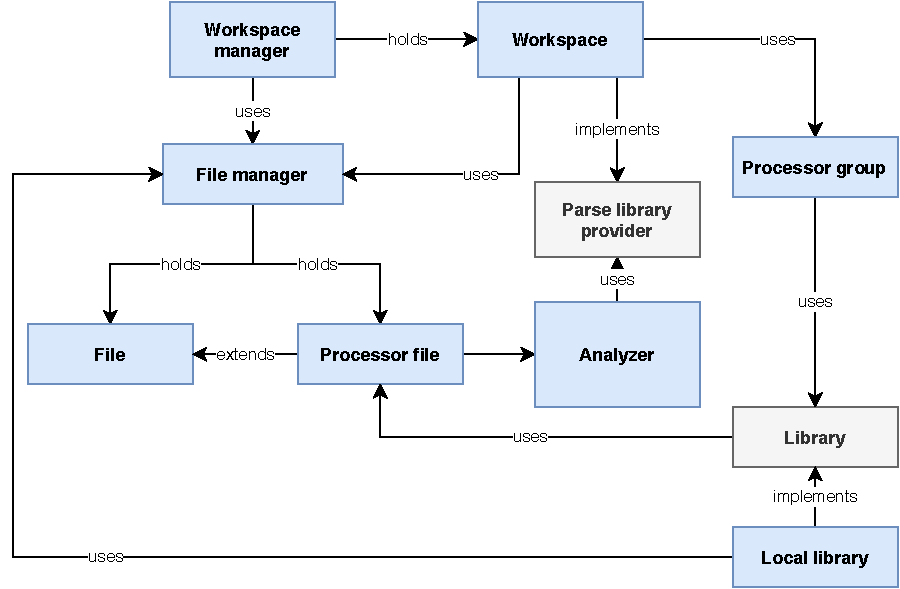
\includegraphics[width=16cm]{img/ws_mngr_arch}
	\caption{Architecture of workspace manager.}
	\label{ws_mngr_arch}
\end{figure}
\end{landscape}


\section{Files}




\section{Libraries resolution}

\section{Diagnosable}

\chapter {Analyzer}

Analyzer's role is to provide a facade over objects and methods that compose this component and provide a simple interface for processing --- analyzing --- a single HLASM source file. The output of the analysis is data for LSP server.

\section{Overview}

\begin{figure}
	\centering
	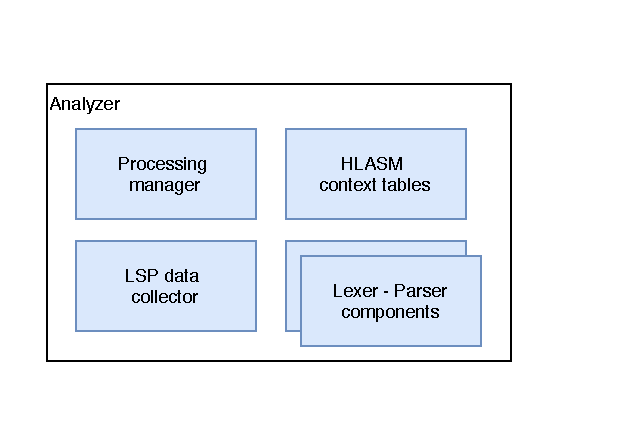
\includegraphics[width=\textwidth / 2]{img/analyzer_arch}
	\caption{The composition of the Analyzer component}
	\label{fig06:analyzer}
\end{figure}

Analyzer is composed of several sub-components all required to properly process the file (see \cref{fig06:analyzer}). 
\begin{itemize}
	\item \emph{LSP data collector} collects and retrieves all LSP information created while processing of the file.
	\item \emph{HLASM context tables} holds information about the context of processed HLASM source code.
	\item Analyzer facades several \emph{Lexer - Parses sub-components} to simplify the interface and ease the use of this component.
	\item \emph{Processing manager} contains the main loop where file is processed.
\end{itemize}

\subsection{Construction}

In order to parse a HLASM file, analyzer is constructed with the following parameters:
\begin{itemize}
	\item \emph{Name and content of the file}
	\item \emph{Parse library provider} -- object responsible for resolving source file dependencies. The dependencies are only discovered during the analysis, so it is not possible to provide the files beforehand.
\end{itemize}

When this constructor is used, analyzer creates HLASM context tables and analyzes the provided source as an open-code. We say that analyzer has \emph{owner semantics}. 
 
Analyzer provides \emph{reference semantics} as well. The provided source is not treated as an open-code, rather as an external file dependency. The constructor of analyzer with reference semantics adds two parameters to the previous one:
\begin{itemize}
	\item \emph{HLASM context tables reference} -- belonging to the owning open-code analyzer.
	\item \emph{Library data} -- states how should be the dependency file further analyzed (see \cref{lab06:lib_data}).
\end{itemize}

This constructor is called within open-code analyzer by it's sub-components when they use Parse library provider.

\vspace{0.5cm}

To sum up, after analyzer is constructed, it analyzes provided source file. In result, it updated HLASM context tables and provides a list of diagnostics linked to the file, highlighting, list of symbol definitions, etc.

\section{LSP data collector}





\section{Processing manager}

\subsection{Instruction interpretation}

Results of the parser component are further analyzed in the processing component. Its most important capabilities are:
\begin{itemize}
	\item Interpretation of CA instructions, which results in modifying the lexer state (moving back and forth in the input file).
	\item Substitution of variable symbols. After the substitution, the statement must be reparsed in the lexer and the parser, since the substitution may completely change its meaning.
	\item Interpretation of assembler instructions
	\item Ordinary symbols resolution
	\item MACRO and COPY expansion.
\end{itemize}

\subsection{Expressions}
overview

they are parsed in grammar, later you give an expression "symbol evaluator" and it returns its value



\subsection{Data definition}

validation and processing purpose
\section{Instruction validation}

One of the essential ways to provide results of the parsing to the user is through error messages. Many of these messages are created in \emph{Instruction checker} which validates the usage of different kinds of instructions.

Instruction checker is an abstract class for various types of instructions. Its \emph{check()} method is being called from the instruction processors~\ref{chap:process} to check whether the specific instruction is used with correct parameters. As assembler and machine instructions have incoherent formats, we derive separate \emph{assembler} and \emph{machine} checkers from the instruction checker. CA instructions do not have a derived checker class as they are all being checked during their interpretation.

The checkers need an access to the definitions of all possible instructions. These instructions are stored statically inside an object called \emph{instruction}. It consists of 4 different containers:
\begin{itemize}
	\item \emph{machine\_instructions} is a map of instruction names to machine instruction object, which contains various data such as format, size or vector of instruction's operands.
	\item \emph{mnemonic\_codes} maps instruction names to their mnemonic code. The mnemonic codes are simplified versions of specific machine instructions, substituting one of the operands by a default value. The mnemonic code objects provides a list of operands to be substituted along with the original instruction name.
	\item \emph{assembler\_instructions} is similar to the machine instructions. However, as the assembler instructions do not have formats, these classes only state minimum/maximum number of operands for specific instruction.~In~\cref{sub:asm_check}, we explain how the assembler instructions are validated.
	\item \emph{ca\_instructions} only contains a list of possible CA instructions.
\end{itemize}

Both assembler and machine checker works in a similar manner:
\begin{enumerate}
	\item Either assembler or machine processor calls the check() method of its respective checker. This method accepts the instruction name, the vector of used operands, the range of statement and the diagnostic collector.
	\item Checker finds the correct instruction based on the provided name and calls the check() method of its instruction class, along with the same parameters as mentioned above.
	\item The instruction itself compares its possible operands with the used operands.
	\item More validations may be necessary, based on the instruction.
	\item In case of mismatch, a diagnostic is added to the passed diagnostic container.
\end{enumerate}

\subsection{Machine instruction checker}

All machine instructions have a precisely defined format which makes the validation based on these formats straightforward. Machine instructions checker operates with machine instructions and their mnemonic codes.

The formats are pretty straightforward. They define several basic operands such as register or address and state which combination of these operands are acceptable. For example, instruction LR has format RR, which means it accepts only 2 arbitrary (but correct) registers. 

\begin{figure}
	\centering
	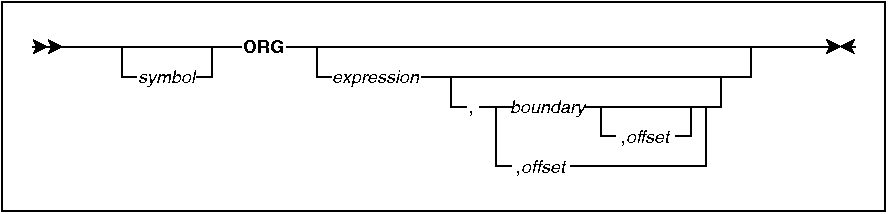
\includegraphics[width=\textwidth]{img/org_diagram}
	\caption{Operand diagram for the ORG instruction.}
	
	\label{fig01:check}
\end{figure}

\subsection{Assembler instruction checker}
\label{sub:asm_check}

Validation of assembler instructions is more complicated as there are no pre-defined formats for them. Each of them is described by custom operand diagrams, which demonstrate the dependencies and relations between operands of a specific instruction. An example of such diagram for the ORG instruction is shown in \cref{fig01:check}. As addition to the basic operands used for machine instructions, each assembler instruction might have its own operands, called keywords.

Due to these irregularities, we derive instruction-specific classes from assembler instruction class. Each of them implements the check() method, to provide the customized checking.

\subsubsection{Data Definition checking}

Data definition is a type of operand in HLASM. It represents data that is assembled directly into object code (see \cref{asm_instrs}).

Since there are many types of data definition, there is a data definition subcomponent of instruction validation. Whenever any component of the project needs information about a data definition operand, it can use this subcomponent. It analyzes each type of data definition and is able to return its length, attributes and check its validity.

Each type is different and many have special conditions that must be met to be valid. That is why there is an abstract class \TT{data\_def\_type\_base}, which has 38 implementations --- one for each type (including type extensions). The types are then available in a static associative map that maps names of types to their representations.




\section{Usage of ANTLR 4}
We have based part of our Analyzer on ANTLR 4 parser generator. ANLTR 4 implements Adaptive $LL(*)$ \cite{parr2014adaptive} parsing strategy.

\subsection{Adaptive $LL(*)$ parsing strategy}
Adaptive $LL(*)$ (or short $ALL(*)$) parsing strategy is a combination of simple, efficient and predictable top-down $LL(k)$ parsing strategy with power of $GLR$ which can handle non-deterministic and ambiguous grammars. 
Authors move the grammar analysis to parse-time. This lets $ALL(*)$ handle any non-left-recursive context-free grammar rules and for efficiency it caches analysis results in lookahead DFA.

Theoretical time complexity can be viewed as a possible downside of $ALL(*)$. Parsing of $n$ symbols takes $O(n^4)$ in theory. In practice, however, $ALL(*)$ seems to outperform other parsers by order of magnitude.

Despite the theoretical $O(n^4)$ time complexity, it appears that the $ALL(*)$ behaves linear on most of the code, with no unpredictable performance or large footprint in practice. In order to support this, authors investigate the parse time vs file size for languages \texttt{C}, \texttt{Verilog}, \texttt{Erlang} and \texttt{Lua} files. They found very strong evidence of linearity on all tested languages (see the original paper for details).

\subsection{ANTLR 4 pipeline}

ANTLR 4, similar to any other conventional parser generator, processes the inputted code as follows: (1) breaks down the source string into tokens using \textit{lexer} (2) \textit{parser} build parse trees. 

This pipeline in ANTLR 4 is broken into following classes: 

\begin{description}
	\item[\texttt{CharStream}] represents input code,
	\item[\texttt{Lexer}] breaks the inputted code into tokens,
	\item[\texttt{Token}] token representation that includes important information like token type, position in code or the actual text,
	\item[\texttt{Parser}] builds parse trees,
	\item[\texttt{TokenStream}] connects the lexer and parser.
\end{description}

\cref{antlr_pipeline} sketches the described pipeline.

\begin{figure}[H]
	\centering
	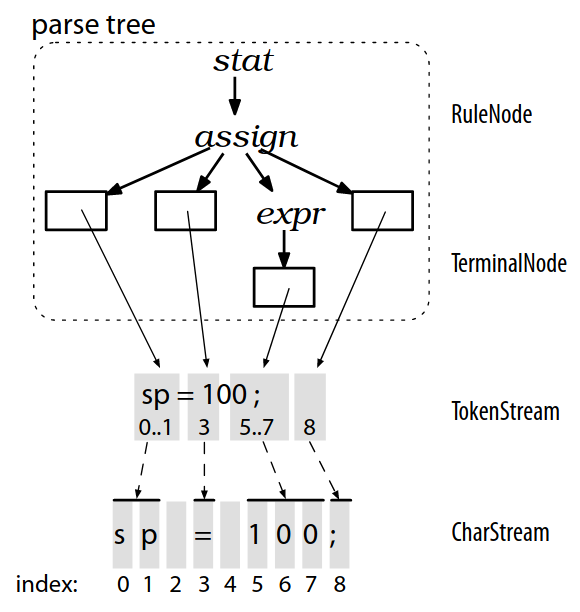
\includegraphics[width=6cm]{img/antlr_pipeline}
	\label{antlr_pipeline}
	\caption{ANTLR 4 pipeline overview. Taken from \cite{parr2013definitive}.}
\end{figure}

\section{Visitor}

We employ ANTLR \emph{visitor} feature during evaluation of CA expressions (see \cref{lab06:expr}). 

The ANTLR 4 first generates \texttt{hlasmparserVisitor} and \texttt{hlasmparserBaseVisitor}. The former is a abstract class, the latter is a simple implementation of the former. Both classes define ``visit'' functions for every grammar rule. A visit function has exactly one argument --- the context of the rule. The simple implementation executes \texttt{visitChildren()}. Our parse-tree visitor --- the \texttt{expression\_evaluator} --- overrides \texttt{hlasmparserBaseVisitor}. In order to evaluate a sub-rule, we call \texttt{visit(ctx->sub\_rule())}, where \texttt{ctx->sub\_rule()} returns the context of the sub-rule. The \texttt{visit()} function matches appropriate function of the visitor based on the context type (for example, \texttt{visit(ctx->sub\_rule())} would call \texttt{visiSub\_rule(..)}).

\section{Lexer}

Lexer's responsibility is to read source string and break it into tokens --- small pieces of text with special meaning. The most important properties of the lexer:
\begin{itemize}
	\item each token has a location in the source text,
	\item has the ability to check whether all characters are valid in the HLASM source,
	\item can jump in the source file backward and forward if necessary (for implementation of instructions like AGO and AIF). Because of this, it is not possible to use any standard lexing tool, and the lexer has to be implemented from scratch.
\end{itemize}

As previously mentioned, we designed a custom lexer for HLASM. We have a number of reasons to do so. HLASM language is complex. It was first introduced several decades ago, and the language was during this long time subjected to development. Such a long period made the HLASM language complex. Also, it contains some aggressive features, for example, \texttt{AREAD} or \texttt{COPY}, that can alter the source code at parse time.

Conventional lexing tools are most often based on regular expressions. As discussed above, there are several difficulties that one must consider designing lexer for this particular language. A regular expression-based lexer would be too difficult or even impossible to design\footnote{One could match separate characters from the input and let the parser or semantic analysis deal with some of the described problems. This drastic solution would cost performance, as parsers are usually more performance demanding.}.

\subsection{Encodings}
Source code encodings differ for the used libraries. All strings are encoded in \texttt{UTF} as follows:

\begin{description}
	\item[\texttt{UTF-8}] LSP string encoding,
	\item[\texttt{UTF-16}] offsets (positions in source code) in LSP,
	\item[\texttt{UTF-32}] ANTLR 4 source code representation.
\end{description}

\subsection{Architecture}

\begin{figure}[H]
	\centering
	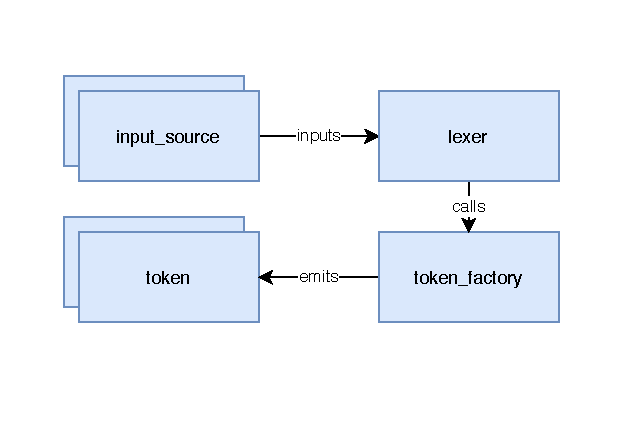
\includegraphics{img/lexer_arch}
	\label{lexer_arch}
	\caption{Lexer architecture overview. Note, there are two \texttt{input\_source}s and there are many \texttt{token}s generated.}
\end{figure}

Beside of the custom lexer, we altered ANTLR's classes \texttt{Token}, \texttt{TokenFactory} and \texttt{ANTLRInputStream}. The reason is to add custom attributes to token that are vital for later stages of the HLASM code analysis (parsing, semantic analyses, etc.). Lexer functionality is implemented in following classes (see \cref{lexer_arch}):



\begin{description}
	
	\item[\texttt{token}] implements ANTLR's class \texttt{Token} and extends it by adding properties important for location of the token within the input stream. As the LSP protocol works with offsets encoded in \texttt{UTF-16} and ANTLR 4 works with \texttt{UTF-32} encoding, we add attributes for \texttt{UTF-16} positions, too.
	
	Token does not carry the actual text from the source but instead references the position in code (unlike \texttt{CommonToken}). Note that the position of a token is vital for further analysis.
	
	\begin{table}
		\centering
		\begin{tabular}{lr}
			\toprule
			\textbf{IGNORED}                                                                     &  sequence of characters ignored in processing \\
			\textbf{COMMENT}                                                                     &                         commentary statements \\
			\textbf{EOLLN}                                                                       &         token signalling the end of statement \\
			\textbf{SPACE}                                                                       &                          a sequence of spaces \\
			\textbf{IDENTIFIER}                                                                  &                             symbol identifier \\
			\textbf{ORDSYMBOL}                                                                   &                    Ordinary symbol identifier \\
			\textbf{PROCESS}                                                                     &                       process statement token \\
			\textbf{NUM}                                                                         &                                        number \\
			\textbf{ATTR}                                                                        & apostrophe that serves as attribute reference \\
			\thead{\textbf{ASTERISK, SLASH, MINUS, PLUS,}\\ \textbf{LT, GT, EQUALS, LPAR, RPAR}} &                             expression tokens \\
			\thead{\textbf{DOT, COMMA, APOSTROPHE,}\\ \textbf{AMPERSAND, VERTICAL}}              &                        special meaning tokens \\ \bottomrule
		\end{tabular}
		\caption{Enumeration of tokens.}
		\label{tab06:tokens}
	\end{table}
	
	Interesting remark of HLASM language complexity is absence of \emph{string} token (see \cref{tab06:tokens}). Lexer does not generate this token due to existence of model statements (see \cref{var_sym}). There, variable symbol can be written anywhere in the statement (even in the middle of the string), what significantly restricts lexer.
	
	\item[\texttt{token\_factory}] produces tokens of previously described custom type \texttt{token}.
	
	\item[\texttt{input\_source}] implements \texttt{ANTLRInputStream} which encapsulates source code. This implementation adds API for resetting, rewinding and rewriting input. 
	
	Beware of the usage of \texttt{UTF} encodings: \texttt{\_data} (source code string) and positions/indices in API are in \texttt{UTF-32}; \texttt{getText} returns \texttt{UTF-8} string.
	
	\item[\texttt{lexer}] is based on ANTLR's \texttt{TokenSource} class. As most lexers, it is also, in principle, a finite state machine. The most important difference compared to conventional FSMs and other lexers is added communication interface that connects the parser and the instruction interpreter with the lexer. Unusual is also input rewinding (to support \texttt{AREAD}, for example), lexing from parallel sources (\texttt{AINSERT} buffer), and some helper API for subsequent processing stages.
	
	Important functions:
	
	\begin{description}
		\item[\texttt{nextToken()}] implements main functionality: lexes and emits tokens. Before lexing, the function uses the right input stream (either the source code or \texttt{AINSERT} buffer if not empty). After choosing the right input source, the lexer emits token is lexed. HLASM introduces \textit{continuation} symbol (an arbitrary non-blank symbol at column 72 by default) that breaks one logical line into two or more lines in code. The end of one logical line indicates \texttt{EOLLN} token. Such token is important for further (syntactic and semantic) analysis.
		
		
		\item[\texttt{create\_token()}] creates token of given type. The lexer's internal state gives the position of the token. 
		
		\item[\texttt{consume()}] consumes character from the input stream and updates lexer's internal state (used in \texttt{create\_token()}).
		
		\item[\texttt{lex\_tokens()}] lexing of most of the token types.
		
		\item[\texttt{lex\_begin()}] up to certain column, the input can be ignored (can be set in HLASM).
		
		\item[\texttt{lex\_end()}] lexes everything after continuation symbol.
		
		
	\end{description}
	
\end{description}


\section{Parser}
\label{lab06:parser}

Parser component takes the tokens produced by lexer from token stream and recognizes HLASM statements.

\subsection{ANTLR overview}

The input to ANTLR is a grammar written in antlr-specific language that specifies the syntax of HLASM language. The framework takes grammar and generates source code (in C++) for a recognizer, which is able to tell whether input source code is valid or not. Moreover, it is possible to assign a piece of code that executes every time a grammar rule is matched by the recognizer to further process the matched piece of code and produce helper structures (statements).

The parser inherits from the recognizer to provide further operations.

\subsection{Parser workflow}

Parser (in code referenced as \TT{parser\_impl}) implements opencode statement provider interface. This means that, according to the statement passing in \cref{lab06:proc_stat}, parser needs to parse each statement in \emph{two steps}:

\begin{enumerate}
	\item Parser calls rule \TT{label\_instr}. It parses label and instruction fields into respective structures. The operand and remark field is stored as string.
	\item After retrieving processing format, parser selects corresponding rule to parse operands. With the rule, it parses remaining string from the previous step.
\end{enumerate}

For the means of parsing remaining strings, parser subcomponent contains actually \emph{two parsers}. The first one parses statement after statement from a source file. The second parses the operands from the string passed by the first parser. 

Operands to have correctly set ranges prior to the source file rather than to the passed string, parser uses \emph{Range provider}. It helps the second parser to have ranges of reparsed operands consistent with the ranges of other fields. It is initialized with the begin location of operand field in the statement and all ranges furtherly created in parsing are adjusted to have correct boundaries.

\subsection{Statement structure}

During parsing of a statement, several structures are created and collected. They are \TT{label\_si, instruction\_si, operand\_si, remark\_si} (\emph{si} as semantic information). They are collected with \TT{collector} and built into \TT{statement\_si} structure.

Label and instruction structures can contain either identifier of a symbol or --- when in model statement --- concatenation of strings and variable symbols. Remark field is simply just a string as it serves as a commentary statement field. Operand field contains list of operands used in the statement. They can be of several formats.

\subsubsection{Concatenation}

A model statement is a statement that contains variable symbol in any of the statement fields. This variable symbol is further to be substituted by an arbitrary string and then re-parsed. Hence, the field is represented by a concatenation of helper structures. The concatenation can be further evaluated to produce the final string.

The helper structures are:
\begin{itemize}
	\item \TT{char\_str} -- character string.
	\item \TT{var\_sym} -- substitutable variable symbol.
	\item \TT{dot}, \TT{equals} -- characters with special meaning.
	\item \TT{sublist} -- by parenthesis enclosed recursive concatenation.
\end{itemize}

\subsubsection{Operand formats}
The statement processor can request parser to retrieve statements with this operand formats:
\begin{itemize}
	\item \emph{machine/assembler/conditional assembly/macro} -- instruction operands. Each type of instruction has it's specific format.
	\item \emph{model} -- operands for model statements. It is a chain of strings and variable symbols.
	\item \emph{deferred} -- operands with not yet known format. Stored as a string.
\end{itemize}

Each operand format has corresponding \emph{operand structure}. They all inherit abstract \TT{operand} and each have various children for different kinds of the operand format (see \cref{fig06:operand_arch}). Assembler and Machine operand structures inherit from \emph{Evaluable operand}. It is a common structure for operand objects that are composed of resolvable objects (see \cref{symbol_dependency_tables}).

\begin{figure}[H]
	\centering
	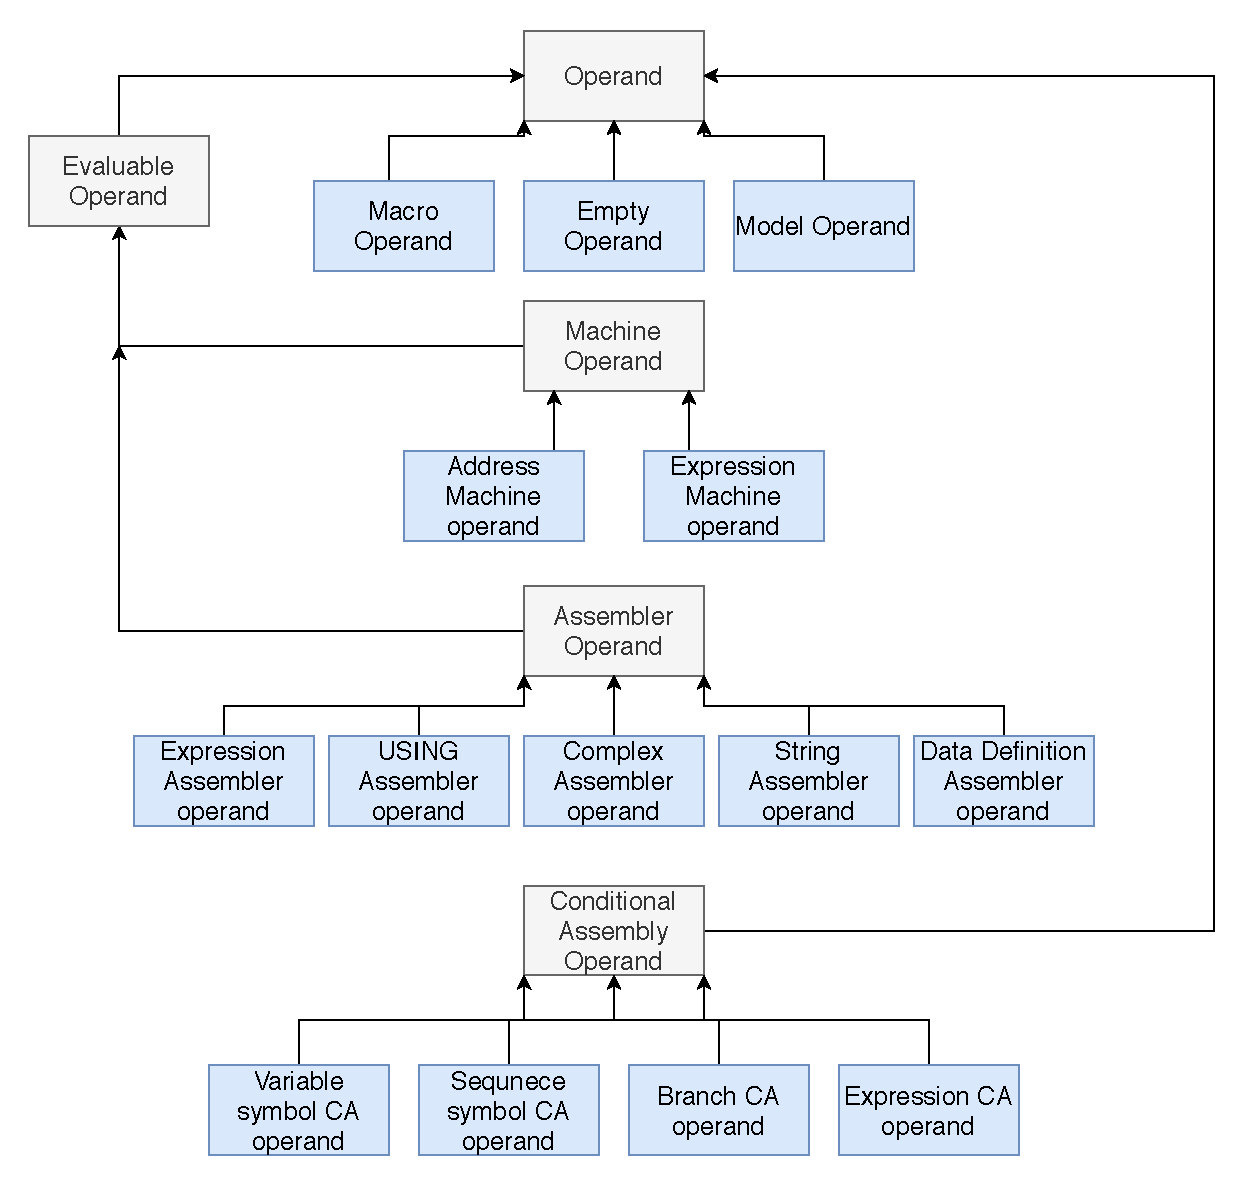
\includegraphics[width=\textwidth]{img/operand_arch}
	\caption{Operand structure inheritance.}
	\label{fig06:operand_arch}
\end{figure}

\subsection{Grammar rules}

Grammar rules describing parser are separated into several files:
\begin{itemize}
	\item \textbf{hlasm\_parser.g4} -- Top level rules are stored here.
	\item \textbf{lookahead\_rules.g4} -- Rules for lookahead mode.
	\item \textbf{label\_field\_rules.g4} -- Rules taking care of label field of statement.
	\item \textbf{instruction\_field\_rules.g4} -- Rules taking care of instruction field of statement.
	\item \textbf{operand\_field\_rules.g4} -- Rules taking care of operand field of statement.
	\item \textbf{macro/machine/assembler/ca/model/deferred\_operand\_rules.g4} -- Concrete operand field rules.
	\item \textbf{ca/asm\_expression\_rules.g4} -- Rules for expressions.
	\item \textbf{data\_def\_rules.g4} -- Rules for data definition.
\end{itemize}

\begin{landscape}
	\begin{figure}
		\centering
		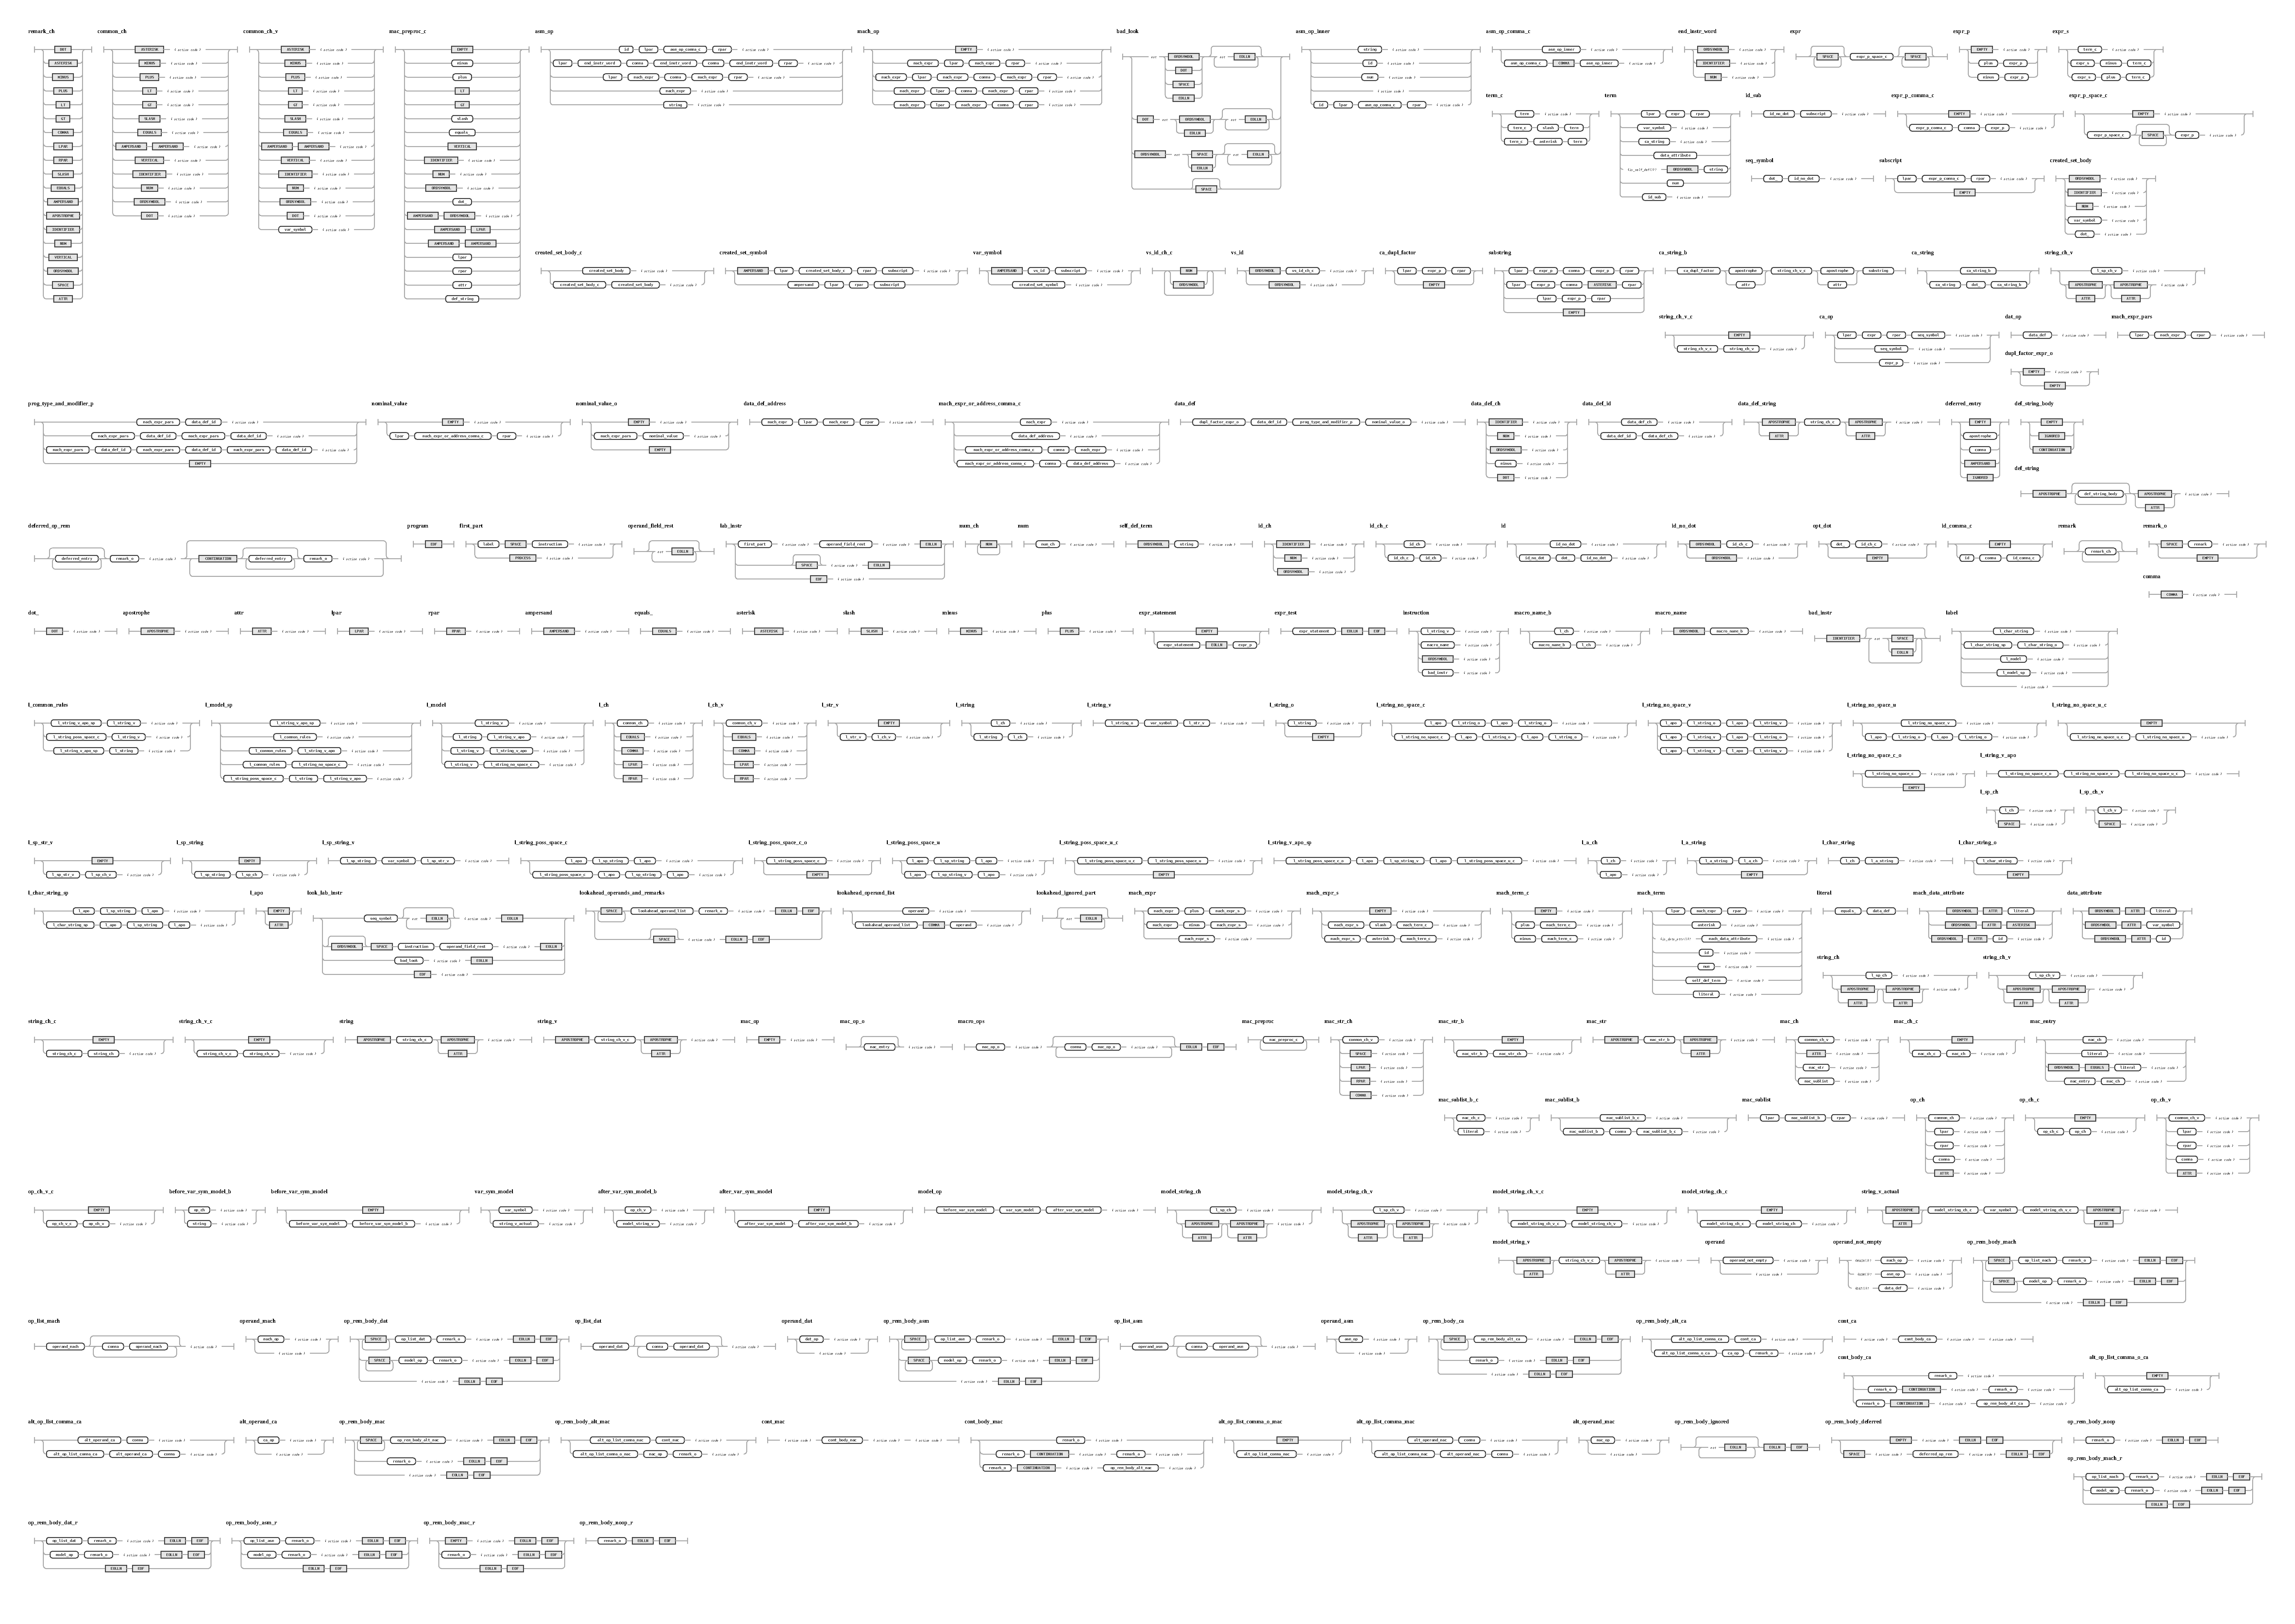
\includegraphics[height=\textheight]{img/grammar}
		\caption{All 193 grammar rules.}
		\label{parser:rules}
	\end{figure}
\end{landscape}


\section{HLASM context tables}

HLASM context tables (in code referred simply as hlasm context) is composition of tables and stacks that describe state of the currently processed open-code (see \cref{fig06:hlasm}). This structure is persistent between source files within an open-code. It is created in analyzer and has the same lifespan. 

It is composed of:

\begin{itemize}
	\item \emph{Macro \& Copy storage} -- stores macro and copy definition definitions.
	\item \emph{ID storage} -- stores symbol identifiers.
	\item \emph{Scope stack} -- stores nested macro invocations and local variable symbols.
	\item \emph{Global variable symbol storage} -- stores global variable symbols.
	\item \emph{Source stack} -- stores nested source files.
	\item \emph{Processing stack} -- stores stack of processings in a source file.
	\item \emph{LSP context}
	\item \emph{Ordinary assembly context} -- encapsulates structures describing Ordinary assembly.
\end{itemize}

\begin{figure}
	\centering
	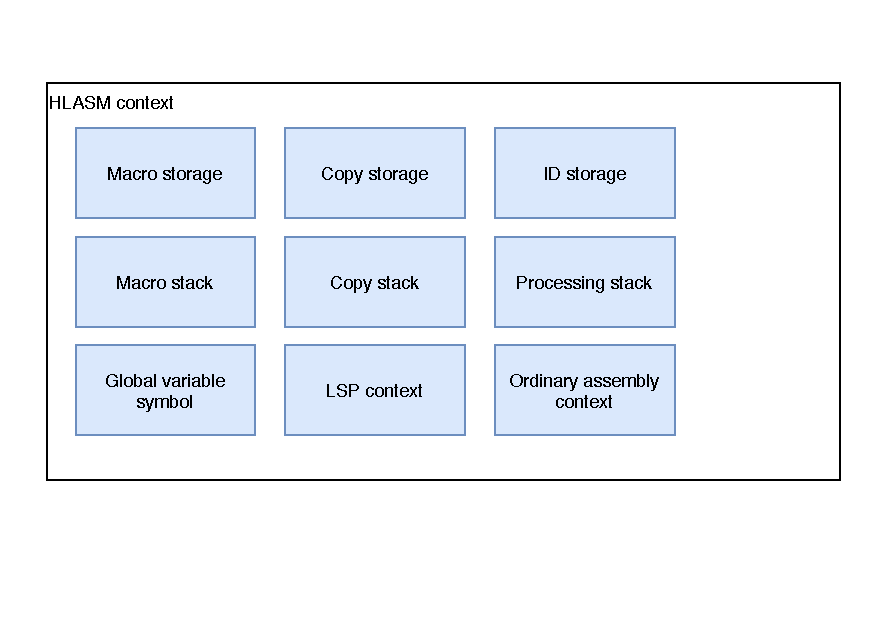
\includegraphics[width=\textwidth / 2]{img/hlasm_arch}
	\caption{The composition of HLASM context tables component}
	\label{fig06:hlasm}
\end{figure}

\subsection{Macros}

HLASM context stores visited macro definitions in the \emph{macro strorage}. 

Macro definition is represented by:
\begin{enumerate}
	\item \emph{Macro identifier}. It identifies the macro.
	\item \emph{Calling parameters}. They are assigned real value when the macro is called.
	\item \emph{Block of statement}. It represents the body of the macro.
	\item \emph{Block of copy nestings}. It is array with one-to-one relation with block of statements. Each entry is a list of in-file locations that represents how much was the statement nested in COPY calls.
	\item \emph{Label storage}. The storage of sequence symbol that occur in the macro definition.
\end{enumerate}

When macro is called, \emph{macro invocation} object is created. It shares the content of a respective macro definition with an exception of calling parameters as they are assigned real value passed with the call. Also, it contains index to the top statement of the invocation.

The macro invocation is stored in the context's \emph{scope stack}.

\subsection{Scope stack}

This stack holds information about the scope of variable symbols (see \cref{lab06:var_sym}). The scope changes when macro is visited. The initial scope is the open-code. 


The stack contains:
\begin{itemize}
	\item In-scope variable symbols.
	\item In-scope sequence symbols.
	\item Pointer to the macro invocation (NULL if in open-code).
	\item Branch counter (for ACTR instruction).
\end{itemize}

\subsection{COPY}

HLASM context stores visited COPY members in the \emph{copy strorage}.

COPY member definition is much more simple than the macro definition as it does not hold any more semantic information than the sequence of statements (the definition itself).

When copy is visited, copy member invocation is created and pushed in the copy stack of last entry of the \emph{source stack}.

\subsection{Source stack and Processing stack}

This stacks are responsible for the nests of opened files (source stack) and what they are opened for (processing stack). As the relation of source entry and processing entry is one-to-many, the information is stored in two arrays rather than one.

When statement processor (see \cref{lab06:sect_proc}) is changed (e.g. macro or copy definition is processed, lookahead is needed, ...), this information is stored in the processing stack. If a new file is opened during this change then source stack is updated as well.

Source stack contains:
\begin{itemize}
	\item \emph{Source file identifier}
	\item \emph{Copy stack} -- the nest of copy calls active for the source file.
	\item \emph{Processed statement location} -- data that locates last processed statement in the source file.
\end{itemize}
Processing stack contains \emph{processing kind}.

The reasoning of organizing this two stacks in such a way is:
\begin{enumerate}
	\item Context has enough information to fully reconstruct the statement.
	\item Easy retrieval of the correct copy stack for copy statement provider.
\end{enumerate} 

\subsection{ID storage}

ID storage holds the string identifiers that are used by the open-code. 
It stores the string and retrieves a pointer. It is guaranteed that if two different strings with the same value are passed to the storage, the resulting pointers are equal.

It simplifies work with IDs and saves space. 

\subsection{Variable symbols}
\label{lab06:var_sym}

In HLASM language, variable symbol is general term for symbols beginning with ampersand. They, however, can be separated into several structures that capture common behavior:

\begin{itemize}
	\item \emph{SET symbols} -- represent HLASM SET symbols.
	\item \emph{System variables} -- represent HLASM system variables.
	\item \emph{Macro parameters} -- represent HLASM macro parameters.
\end{itemize}

They inherit common abstract ancestor \emph{variable symbol}. SET symbols are further divided into \emph{SETA}, \emph{SETB} and \emph{SETC} symbols. Macro parameters are divided into \emph{keyword} and \emph{positional} parameters (see \cref{fig06:var}).

\begin{figure}
	\centering
	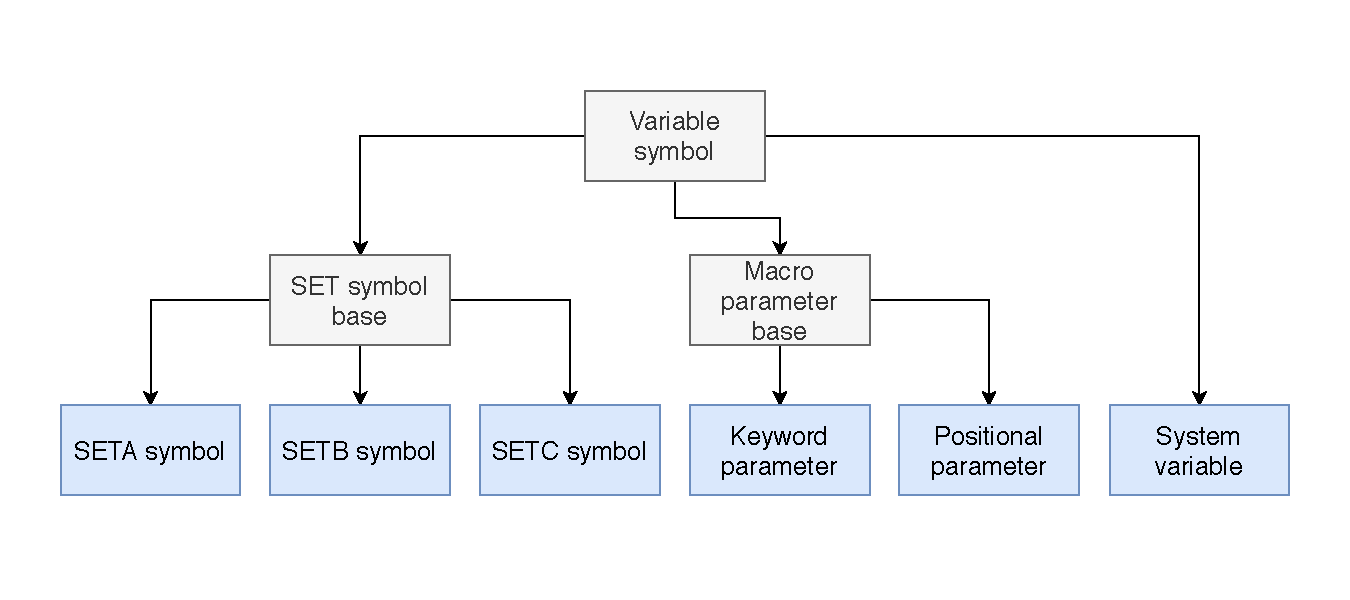
\includegraphics[width=\textwidth]{img/variable_arch}
	\caption{The inheritance of variable symbols.}
	\label{fig06:var}
\end{figure}

\subsection{LSP context}

The LSP context serves as the collection point for the data needed to answer the LSP requests. It is a part of the HLASM context to be able to pass on the LSP data between different parsed files.

The LSP data collector stores its values inside the LSP context tables. More about the collection of the data and their values can be found in~\cref{lsp_data}.

\subsection{Ordinary assembly context}

The above described structures aimed to describe the high-level part of the language (code generation). As we move closer to the resulting object code of the source file, the describing structures get complicated. Therefore, HLASM context contains object storing just this part of the processing.

\begin{figure}
	\centering
	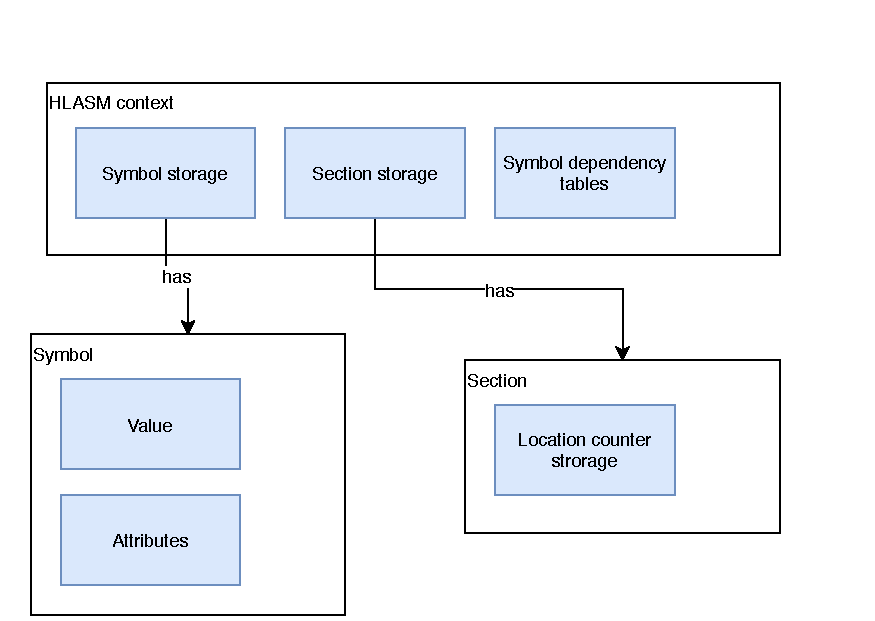
\includegraphics[width=\textwidth / 2]{img/ord_ctx_arch}
	\caption{The composition of Ordinary assembly context}
	\label{fig06:ord_ctx}
\end{figure}

Ordinary assembly context consists of three main components (see \cref{fig06:ord_ctx}):
\begin{enumerate}
	\item \emph{Symbol storage}. Stores ordinary symbols (see \cref{ord_sym}).
	\item \emph{Section storage}. Has notion of all generated sections, each section containing its location counters.
	\item \emph{Symbol dependency tables}. Contains yet unresolved dependencies between symbols prior to the currently processed instruction.
\end{enumerate}

\subsubsection{Symbol}

This class represents HLASM Ordinary symbol (see \cref{ord_sym}). Besides its identifier and location, symbol contains \emph{value} and \emph{attributes} components.

\paragraph*{Value} can be assigned \emph{absolute} or \emph{relocatable} values. With addition to that, it can also be assigned empty value stating that symbol is not yet defined.

\paragraph*{Attributes} structure holds symbol attributes like type, length, scale and integer.

\subsubsection{Section}

Section is a structure representing HLASM section (created by CSECT, DSECT, ...). It contains enumeration \emph{section kind} describing type of the section prior to the used instruction. The structure also holds \emph{location counter storage} with defined location counters.

\subsubsection{Location counter}

This structure contains data and operations for one location counter. The data is stored in helper sub-structure \emph{location counter data}.

\paragraph*{Location counter data} is a structure defining current value of the location counter. It consists of:
\begin{itemize}
	\item \emph{Storage} stating total number of bytes occupied by the location counter.
	\item Vector of \emph{spaces}, block of bytes with yet not known length.
	\item Vector of \emph{storage} between each space.
	\item Currently valid \emph{alignment} (used when data contain spaces).
\end{itemize}

The location counter value is transformable into a relocatable value. It is represented by structure \emph{address}.

\paragraph*{Address} consists of:
\begin{itemize}
	\item Array of \emph{bases}. A base is a beginning of a corresponding section. They serve as points of reference for the address.
	\item Array of \emph{spaces} that are present in the address. 
	\item \emph{Offset} from the bases.
\end{itemize}

The common composition of an address is one base section (as the start of the address) and value of storage (as the offset from it).

The need for the whole array of bases is because addresses from different sections can be arbitrarily added or subtracted. This information is needed as the correct sequence of arithmetic operations can reduce number of bases (even spaces) to zero and create absolute value. This value can be later used in places where a relocatable value would be forbidden.

\paragraph*{Space} is block of bytes with yet not known length. It is created in the active location counter when execution of counter's operation can not be performed due to non previously defined ordinary symbols. See the different kind of spaces and the reason of creation in  the \cref{tab06:space}.

\begin{table}
	\centering
	\begin{tabular}{lr}
		\textbf{Space Kind} &                                          \textbf{Creation} \\ \toprule
		Ordinary            &            when instruction outputs data of unknown length \\
		LOCTR begin         &  when defining more than one location counter in a section \\
		Alignment           &   when current alignment is unknown due to previous spaces \\
		LOCTR set           &     when moving counter's value to the address with spaces \\
		LOCTR max           & when moving counter's value to the next available location \\
		LOCTR unknown       &     when moving counter's value to the yet unknown address \\ \bottomrule
	\end{tabular}
	\caption{Different kinds of spaces and reasons of creation.}
	\label{tab06:space}
\end{table}


When a space length becomes known, all addresses containing the spaces need to be updated (remove the space and append offset). Therefore, space structure contains an array of address listeners. Hence, when an address is assigned a relocatable value that contains the space, the address is added to its array. This serves as an easy point of space resolving.

\vspace{0.5cm}

ORG instruction can arbitrarily move location counter's value forward and backward. With addition to that, ORG can also order location counter to set it's value to the next available value (the lowest untouched address, see \cref{loctr}). Combining this with the possible spaces creation, location counter holds an array of the location counter data to properly set the next available value.

\subsubsection{Symbol dependency tables}
\label{symbol_dependency_tables}
HLASM forbids cyclic symbol definition. This component maintains dependencies between symbols and detects possible cycles.
Let us describe the main components of dependency resolving:

\paragraph*{Dependant} is a structure used in the symbol dependency tables. It encapsulates objects that can be dependent on another. Dependant object can be a \emph{symbol}, \emph{symbol attribute} and \emph{space}.

\paragraph*{Dependable} If an object can contain dependencies, it implements \emph{dependable} interface. The interface has a method to retrieve an structure holding the respective \emph{dependants}. 

\paragraph*{Resolvable} interface adds up to the dependable interface. It is implemented by objects that serve as values assignable to \emph{depednants}. It provides methods to return \emph{symbol value} with help of the dependency solver. 

\paragraph*{Dependency solver} is an interface that can return value of the symbol providing its identifier. It is implemented by Ordinary assembly context.

\vspace{0.5cm}

Having described building blocks, we can move to the symbol dependency tables composition:
\begin{itemize}
	\item \emph{Dependency map}
	\item \emph{Dependency sources map}
	\item \emph{Postponed statements storage}
\end{itemize}

\paragraph*{Dependency map} is the primary storage of dependencies. It has \emph{dependants} as keys and \emph{resolvables} as values. The semantics for pair \emph{(D,R)} is that D is dependent on the dependencies from R. Each time new dependency is added, this map is searched for cycle.

\paragraph*{Dependency sources map} serves as a source objects storage of a resolvable in the dependency map. Hence for the pair \emph{(D,R)} from dependency map, source object of \emph{R} is in the dependency source map under the key \emph{D}. 

The source objects are statements. To be more specific, as one statement can be a source for more distinct resolvables, this source map only stores pointers to the \emph{postponed statements storage}.

\paragraph*{Postponed statements storage} holds statements that are sources of resolvables in dependency map. The reason they are stored is that they can not be checked yet as they contain dependencies. Therefore, they are postponed in the storage until all of the dependencies are resolved. Then they are passed to the respective checker.





\chapter{Macro Tracer}

Macro tracer allows the user to track how HLASM source code is assembled in experience similar to common debugging tools. The user is able to see step by step how CA instructions are interpreted and how macros are expanded.

It is achieved by implementing the Debug Adapter Protocol. The protocol itself is implemented in the language server component, which uses the macro tracer component.

\section{DAP functionality mapping}

The DAP was originally designed to communicate between IDE or editor and debugger or debug adapter. For example, when debugging a C++ application in Visual Studio Code, the editor communicates through DAP with a debugger which is attached to a compiled C++ application.  Contrary to this, macro tracer does not run with compiled binary, it only uses analyzer to simulate the compilation process of high level assembler.

However even though we are not implementing real debugger, it makes very good sense to use debugging interface for tracing the simulation.
\begin{itemize}
	\item \textbf{Instruction pointer} Instruction pointer is commonly showed in debuggers by highlighting line of code which is going to be executed next. This is applicable to HLASM without change, since all the instructions are processed one by one in well defined order.
	\item \textbf{Breakpoints} The user can set a breakpoint when he is interested in tracing only particular section of code. The compilation simulation will stop when it reaches line with breakpoint.
	\item \textbf{Continue} The user can restart stopped simulation by using continue function just as in any debugger.
	\item \textbf{Step in and step over} In debuggers, it is possible to use step in / step over functions to debug implementation of subroutines or skip it and continue after the application returns from the subroutine. In HLASM, this can be applied to macros and COPY instructions: if the user is interested in what happens inside a macro or COPY file, he can use step in. Step over skips to the next instruction in the same file.
	\item \textbf{Variables} The same way common debuggers show values of runtime variables, the macro tracer uses the same functionality to show values of set symbols, macro parameter values and ordinary symbols. It is also possible to visualize attributes of symbols.
	\item \textbf{Call stack} Call stack makes sense with macro tracer too. It can show the stack of currently processed macros and COPY files. Moreover, macros have local set symbols and parameters, so each stack frame may show a different set of valid variables.
\end{itemize}
All described functionality (and more) is supported by the DAP. 
  
\section{Macro tracer architecture}
\begin{figure}
	\centering
	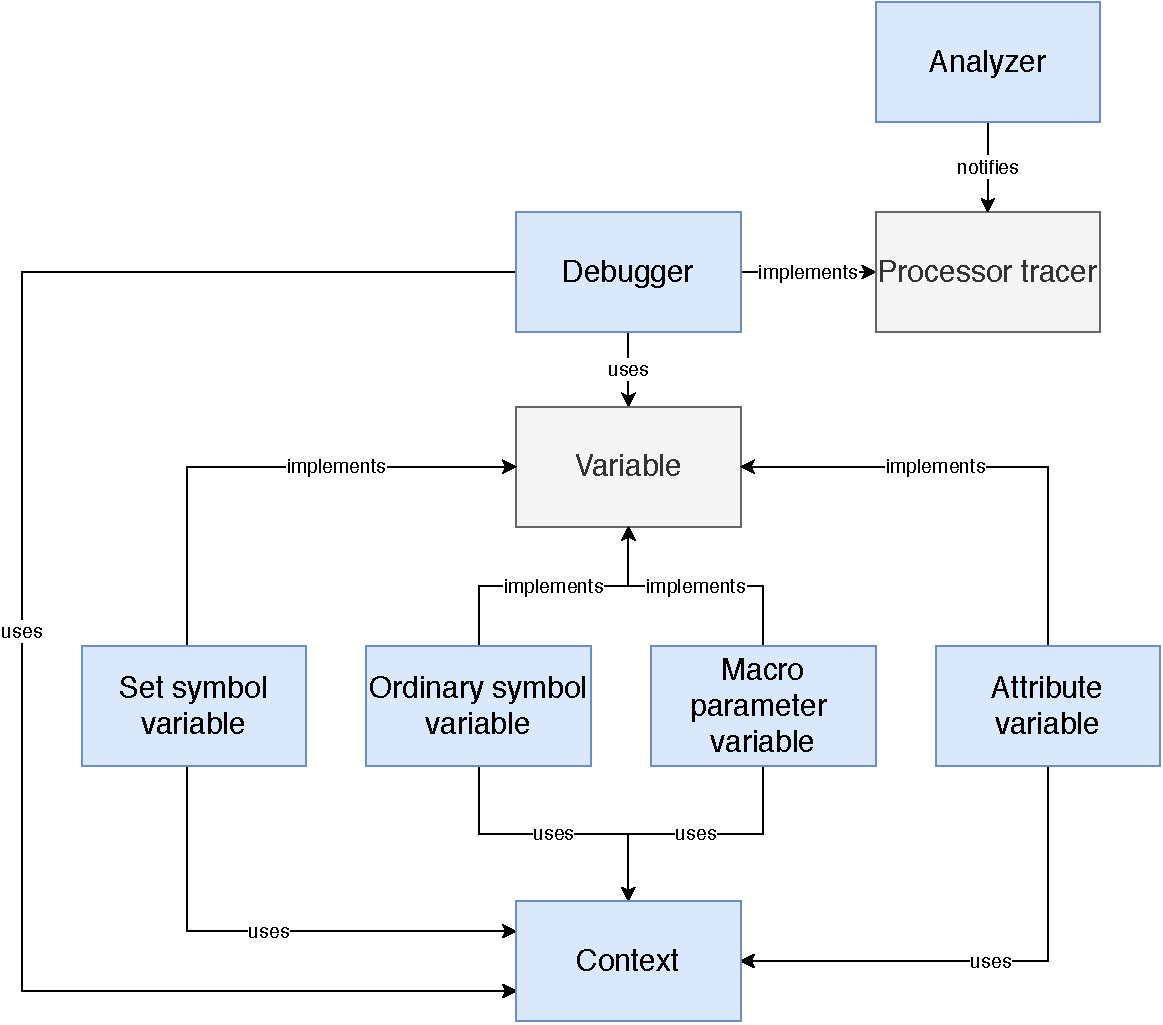
\includegraphics[width=\textwidth]{img/macro_tracer_arch}
	\caption{Architecture of macro tracer.}
	\label{macro_tracer_arch}
\end{figure}

Macro tracer architecture is shown in \cref{macro_tracer_arch}.

Debugger is a class that encapsulates all macro tracer functionality. It starts standard analysis that is provided by the analyzer component in a special thread. The debugger implements processor tracer interface which allows it to receive a notification every time when a statement is about to be processed.

It is also debugger responsibility to extract data from the context used by the analyzer and transform them to a form compatible with DAP.

Debugger uses interface variable which represents a variable as it is shown to the user --- most importantly it is a name-value pair. The variable interface has four implementations:
\begin{itemize}
	\item Set symbol variable
	\item Ordinary symbol variable
	\item Macro parameter variable
	\item Attribute variable
\end{itemize}
Each of the first three represent a HLASM symbol of certain type. They adapt the context representation of the symbols to DAP variables.

Attribute variable represents attributes of all types of symbols. It does not access context, it is only used by the rest of variables to show their attributes.

\section{Debugger}


The debugger component is the core of macro tracer implementation. When the user starts debugging, method \TT{launch} is called from the language server component. The debugger creates analyzer and starts analysis in a separate thread. The debugger implements processor tracer interface which only has one method \TT{statement}. The analyzer calls the \TT{statement} method every time when next statement is about to be processed.

This implementation makes it possible for debugger to stop the analysis using conditional variable. When it sees fit (e.g. when a breakpoint was hit), the debugger can put the thread to sleep and wait for further user interaction. At the same time, it notifies the language server through debug event consumer interface that the analyzer has stopped.

There are three important structures in DAP.
\begin{itemize}
	\item \textbf{Stack frame} Stack frame is one item in call stack. Each frame has name that is shown to the user and points to a line in source code. In macro tracer, each frame points either to the next instruction, to macro call or a COPY instruction.
	\item \textbf{Scope} Each stack frame may have scopes. A scope is simply a group of variables used to make them organized for the user. Macro tracer uses three scopes: Local variables, global variables and ordinary symbols.
	\item \textbf{Variable} Each scope has any number of variables. Each variable has a name and value. They may be further structured and have additional child variables. So DAP can be used to present arbitrary tree of variables to the user. \Cref{dap_nested_variables} shows an example regarding nested macro parameters.

\end{itemize}

\begin{listing}
	
	\begin{verbatim}
	MAC (foo,((bar,ex),am),ple,(lorem,ipsum))
	
	1: foo
	2: ((bar,ex),am)
	1: (bar,ex)
	1: bar
	2: ex
	2: am
	3: ple
	4: (lorem,ipsum)
	1: lorem
	2: ipsum
	
	\end{verbatim}
	\caption{An example how macro tracer leverages DAP nested variables. First line shows a macro call with a parameter. HLASM treats such parameters as nested arrays. Second part shows how such parameter is shown in VS Code using nested variables}
	\label{dap_nested_variables}
\end{listing}

While the thread is stopped, the editor sends requests to display informations about current context. It is the debugger responsibility to extract list of stack frames from the context, return list of scopes for each stack frame and list of variables for each scope. It does not have to deal with complexity of different types of set symbols and macro parameters, that is done by implementations of the variable interface.



\chapter{VS Code extension}

The frontend of the project is implemented as an extension to a modern IDE instead of creating a completely new GUI. This approach has the advantage of providing a familiar environment and workflow that the developers are used to.

There are several IDEs that currently (natively) support LSP, such as \emph{Eclipse Che} and \emph{Eclipse IDE}, \emph{vim8}, \emph{Visual Studio} and \emph{Visual Studio Code} and many more. Others, for example \emph{IntelliJ}, have plugins which add the support for LSP.

Our IDE choice is \emph{Visual Studio Code}, due to its popularity and lightweight design. Conveniently, \emph{Theia}, a web-based IDE, supports VSCode extensions, therefore our plugin works with \emph{Theia} as well.

\section{Standard LSP Extension}

The core of the extension is an activation event which starts the plugin for VSCode.

Upon activation, \emph{Language Client} and \emph{Language server}~\ref{chap:lang_server} are started as child processes of VSCode and a pipe is open for their communication. The LSP communication and its features are handled by the \emph{vscodelc} package. 

To be independent of pipes, we have added an option to use TCP, which assigns a random free port for TCP communication.

\section{DAP Extension}

\emph{Macro Tracer}~\ref{chap:macro_tracer} is implemented using DAP, which is also supported out-of-the-box by VSCode. Similarly to LSP TCP support, we dynamically assign a random free port for DAP communication during the activation.

\section{Additions}

Several features are added to the extension to simplify work with HLASM in modern editors. These additions are specific for Visual Studio Code (and Theia) and are not a part of the LSP specification.

\subsection{Language Detection}

The usual workflow with the extension begins with downloading HLASM source codes from mainframe. Typically, these files will not have any file extension and even if they do, they might differ across various products.

To cope with this problem, there are several mechanisms that help the user to recognize the file as HLASM automatically.

\subsubsection{Macro Detection}

Each file starting with line \emph{MACRO} (arbitrary number of whitespace before and after) is recognized as HLASM.

\subsubsection{Configuration Files Detection}

Every file either defined as a program or as a part of a processor group is recognized as HLASM.

\subsubsection{Wildcards}

Configuration file \emph{pgm\_conf.json} contains a field \emph{alwaysRecognize}, which consists of user-defined wildcards. Every file that satisfies at least one of these wildcards is recognized as HLASM.

\subsubsection{Automatic Language Detection}

Whenever a file is open, its contents are scanned line by line. Whether a file is HLASM or not is determined by a ratio (\# HLASM lines)/(\# all lines).

Recognition is mostly based on a pre-defined set of most used instructions. If a line correctly uses one of these instructions, it is counted as a HLASM line. Continued line of a HLASM line is also a HLASM line.
Moreover, a HLASM line must not exceed 80 characters.

Comment lines or empty lines are skipped and not counted. 

We tested the detection on ~25.000 HLASM files. The best results were observed using 4/10 ratio, with 88\% true positive recognition and 95\% true negative recognition. 

Because of the indeterminate outcomes, this method is meant to be used as a fall-back in case all previous methods do not suffice.

All detection layers are visualized in \cref{fig08:lang}.

\subsection{Continuation Handling}

Due to historical reasons, HLASM has a 80 character-per-line limitation. Modern languages do not enforce such restriction and therefore IDEs such as VSCode allow the user to extend their lines freely. This causes 2 major inconveniences.

First of all, the user must add the continuation character on a very specific column manually. Secondly, each time the user types in between continuation character and the instruction/parameters, the continuation character is pushed from its requisite position and needs to be moved back, again manually.

To improve this behavior, the extension offers an option to activate \emph{Continuation Handling}. 

The first problem is solved by adding two editor commands \emph{insertContinuation} and \emph{deleteContinuation}, which, when invoked, insert/delete the continuation character on its correct position.

To improve the second problem, the option overrides standard VSCode commands, commonly used when working in editor such as \emph{type}, \emph{deleteLeft}, \emph{deleteRight}, \emph{cut} and \emph{paste}. They offset the continuation character by removing/adding whitespaces in front of it.


\subsection{Configuration Prompt}

If the workspace contains a HLASM file, but does not have configurations, the user is prompted to create them. The warning message also offers an option to create templates for them.

\subsection{HLASM Semantic Highlighting}

In case of HLASM, a semantic (server-side) highlighting is desired. The multi-layered nature of the language causes that in quite common scenarios, specific parts of the code can be highlighted if and only if some previous part was completely processed (parameters for instructions, skipped code thanks to code generation, defined macros, continuations, etc...).

Based on the open pull request to the VSCode Language Server \footnote{https://github.com/microsoft/vscode-languageserver-node/pull/367/files}, we added \emph{semanticHighlighting} as an extra feature of LSP. This feature works in a very similar manner, implementing the LSP interfaces that VSCode provides. It works as a notification from the server to the client, containing ranges of code and their respective tokens (e.g. instruction, label, parameter, comment,..). 

On top of that, we extended \emph{semanticHighlighting} to \emph{ASMsemanticHighlighting}, which adds the ability to notify the client about new code layout, specifically start, continuation and continue columns. These fields can be set in the HLASM code (via ICTL instruction) and are required for the \emph{Continuation Handling} feature to work properly. Our client-server communication is shown in \cref{fig08:lsp}.


\begin{figure}
	\centering
	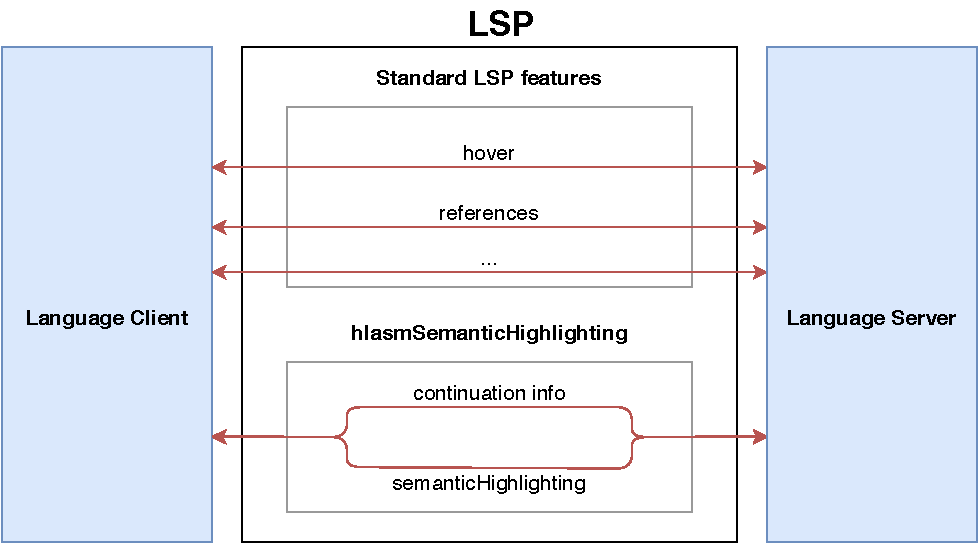
\includegraphics[width=\textwidth]{img/lsp_addition}
	\caption{The addition of semantic highlighting to the LSP communication.}
	
	\label{fig08:lsp}
\end{figure}

\begin{figure}
	\centering
	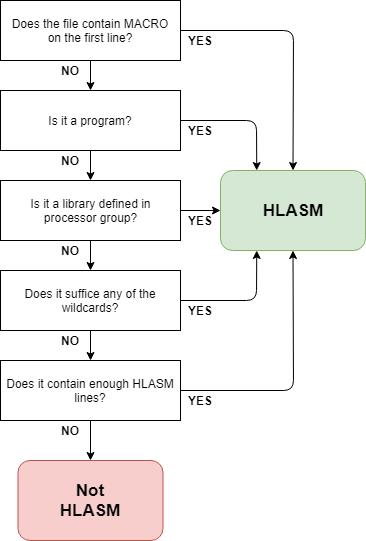
\includegraphics[width=10cm]{img/lang_detection}
	\caption{Language Detection layers.}
	
	\label{fig08:lang}
\end{figure}

\chapter{Build instructions}

In this chapter, we describe how to build the project on different platforms. We only describe methods that we use and are guaranteed to work, but other platforms and versions may work as well.

The results of a build are:
\begin{itemize}
	\item executables \TT{library\_test} and  \TT{server\_test} that can be executed to test the build
	\item a Visual Studio Code extension packed into a VSIX file
\end{itemize}
After the project has been built, the results can be found in bin subdirectory of the build folder.

\section{Prerequisites}
\label{prereq}
In order to build the project on any platform, following software needs to be installed:

\begin{itemize}
	\item CMake 3.10 or higher
	\item C++ compiler with support for C++17
	\item Java Development Kit (JDK) 8 or higher 
	\item Maven
	\item Git 
	\item npm
\end{itemize}

CMake is the build system we use, we use also the C++17 standard. JDK and Maven are needed because of ANTLR4, since we build it from source. Git is needed to download those sources. Npm handles the typescript part of our project.

\section{Windows}

On windows, we use Visual Studio Community 2019. We also have VS configurations for building and testing the project in WSL.

It is also possible to build the project from command line:
\begin{verbatim}
mkdir build && cd build
cmake ../
cmake --build .
\end{verbatim}

\section{Linux}

In addition to the prerequisites listed in \cref{prereq}, linux build has two more prerequisites:

\begin{itemize}
	\item pkg-config
	\item UUID library
\end{itemize}


We build the project for Ubuntu 18.04 and for the Alpine linux.
\subsection{Ubuntu}
On Ubuntu 18.04 the following commands install all prerequisites and then build the project into \TT{build} folder:

\begin{verbatim}
apt update && sudo apt install cmake g++-8 uuid-dev npm default-jdk
                       pkg-config maven
mkdir build && cd build
cmake -DCMAKE_C_COMPILER=gcc-8 -DCMAKE_CXX_COMPILER=g++-8 ../
cmake --build .
\end{verbatim}


\subsection{Alpine linux}

The build works on Alpine linux version 3.10. The following commands install all prerequisites and then build the project into \TT{build} folder:
\begin{verbatim}
apk update && apk add linux-headers git g++ cmake util-linux-dev npm ninja
                      pkgconfig openjdk8 maven
mkdir build && cd build
cmake ../
cmake --build .
\end{verbatim}


\section{Mac OS}
We have only built the project on MacOS 10.14. In order to successfully build, we require LLVM 8 (it can be installed by using homebrew).

The project can be built with a snippet like this:
\begin{verbatim}
mkdir build && cd build
cmake -DCMAKE_C_COMPILER=clang -DCMAKE_CXX_COMPILER=clang++
      -DLLVM_PATH=<path-to-llvm-installation> ../
cmake --build .
\end{verbatim}
For instance, on my computer, the path to LLVM is this: \TT{/usr/local/opt/llvm\@8}


\bibliography{biblio} 
\bibliographystyle{apalike}

\begin{appendices}


%\includepdf[pages=-,fitpage=true]{all_arch.pdf}

\newenvironment{foldoutfloat}{%
	\eject\pdfpageheight=52cm\pdfpagewidth=40cm
	\newgeometry{margin=1in}
	\textwidth=15in
	\begin{figure}[p]
	}{%
	\end{figure}
	\clearpage % otherwise it will float to another, non-resized page
	\eject\pdfpageheight=11in\pdfpagewidth=8.5in
	\restoregeometry
}%

\newenvironment{foldoutfloatlandscape}{%
	\eject\pdfpageheight=40cm\pdfpagewidth=52cm
	\newgeometry{margin=1in}
	\textwidth=15in
	\begin{figure}[p]
	}{%
	\end{figure}
	\clearpage % otherwise it will float to another, non-resized page
	\eject\pdfpageheight=11in\pdfpagewidth=8.5in
	\restoregeometry
}%

\begin{foldoutfloat}
	\chapter{Architecture of the project}
	\label{all_arch}
	\thispagestyle{empty}

	\includegraphics[width=35cm]{img/all_arch}
	\caption{Architecture of the whole project}
\end{foldoutfloat}

\begin{foldoutfloatlandscape}
	\chapter{Parser grammar}
	\label{parser_rules}
	\thispagestyle{empty}
	
	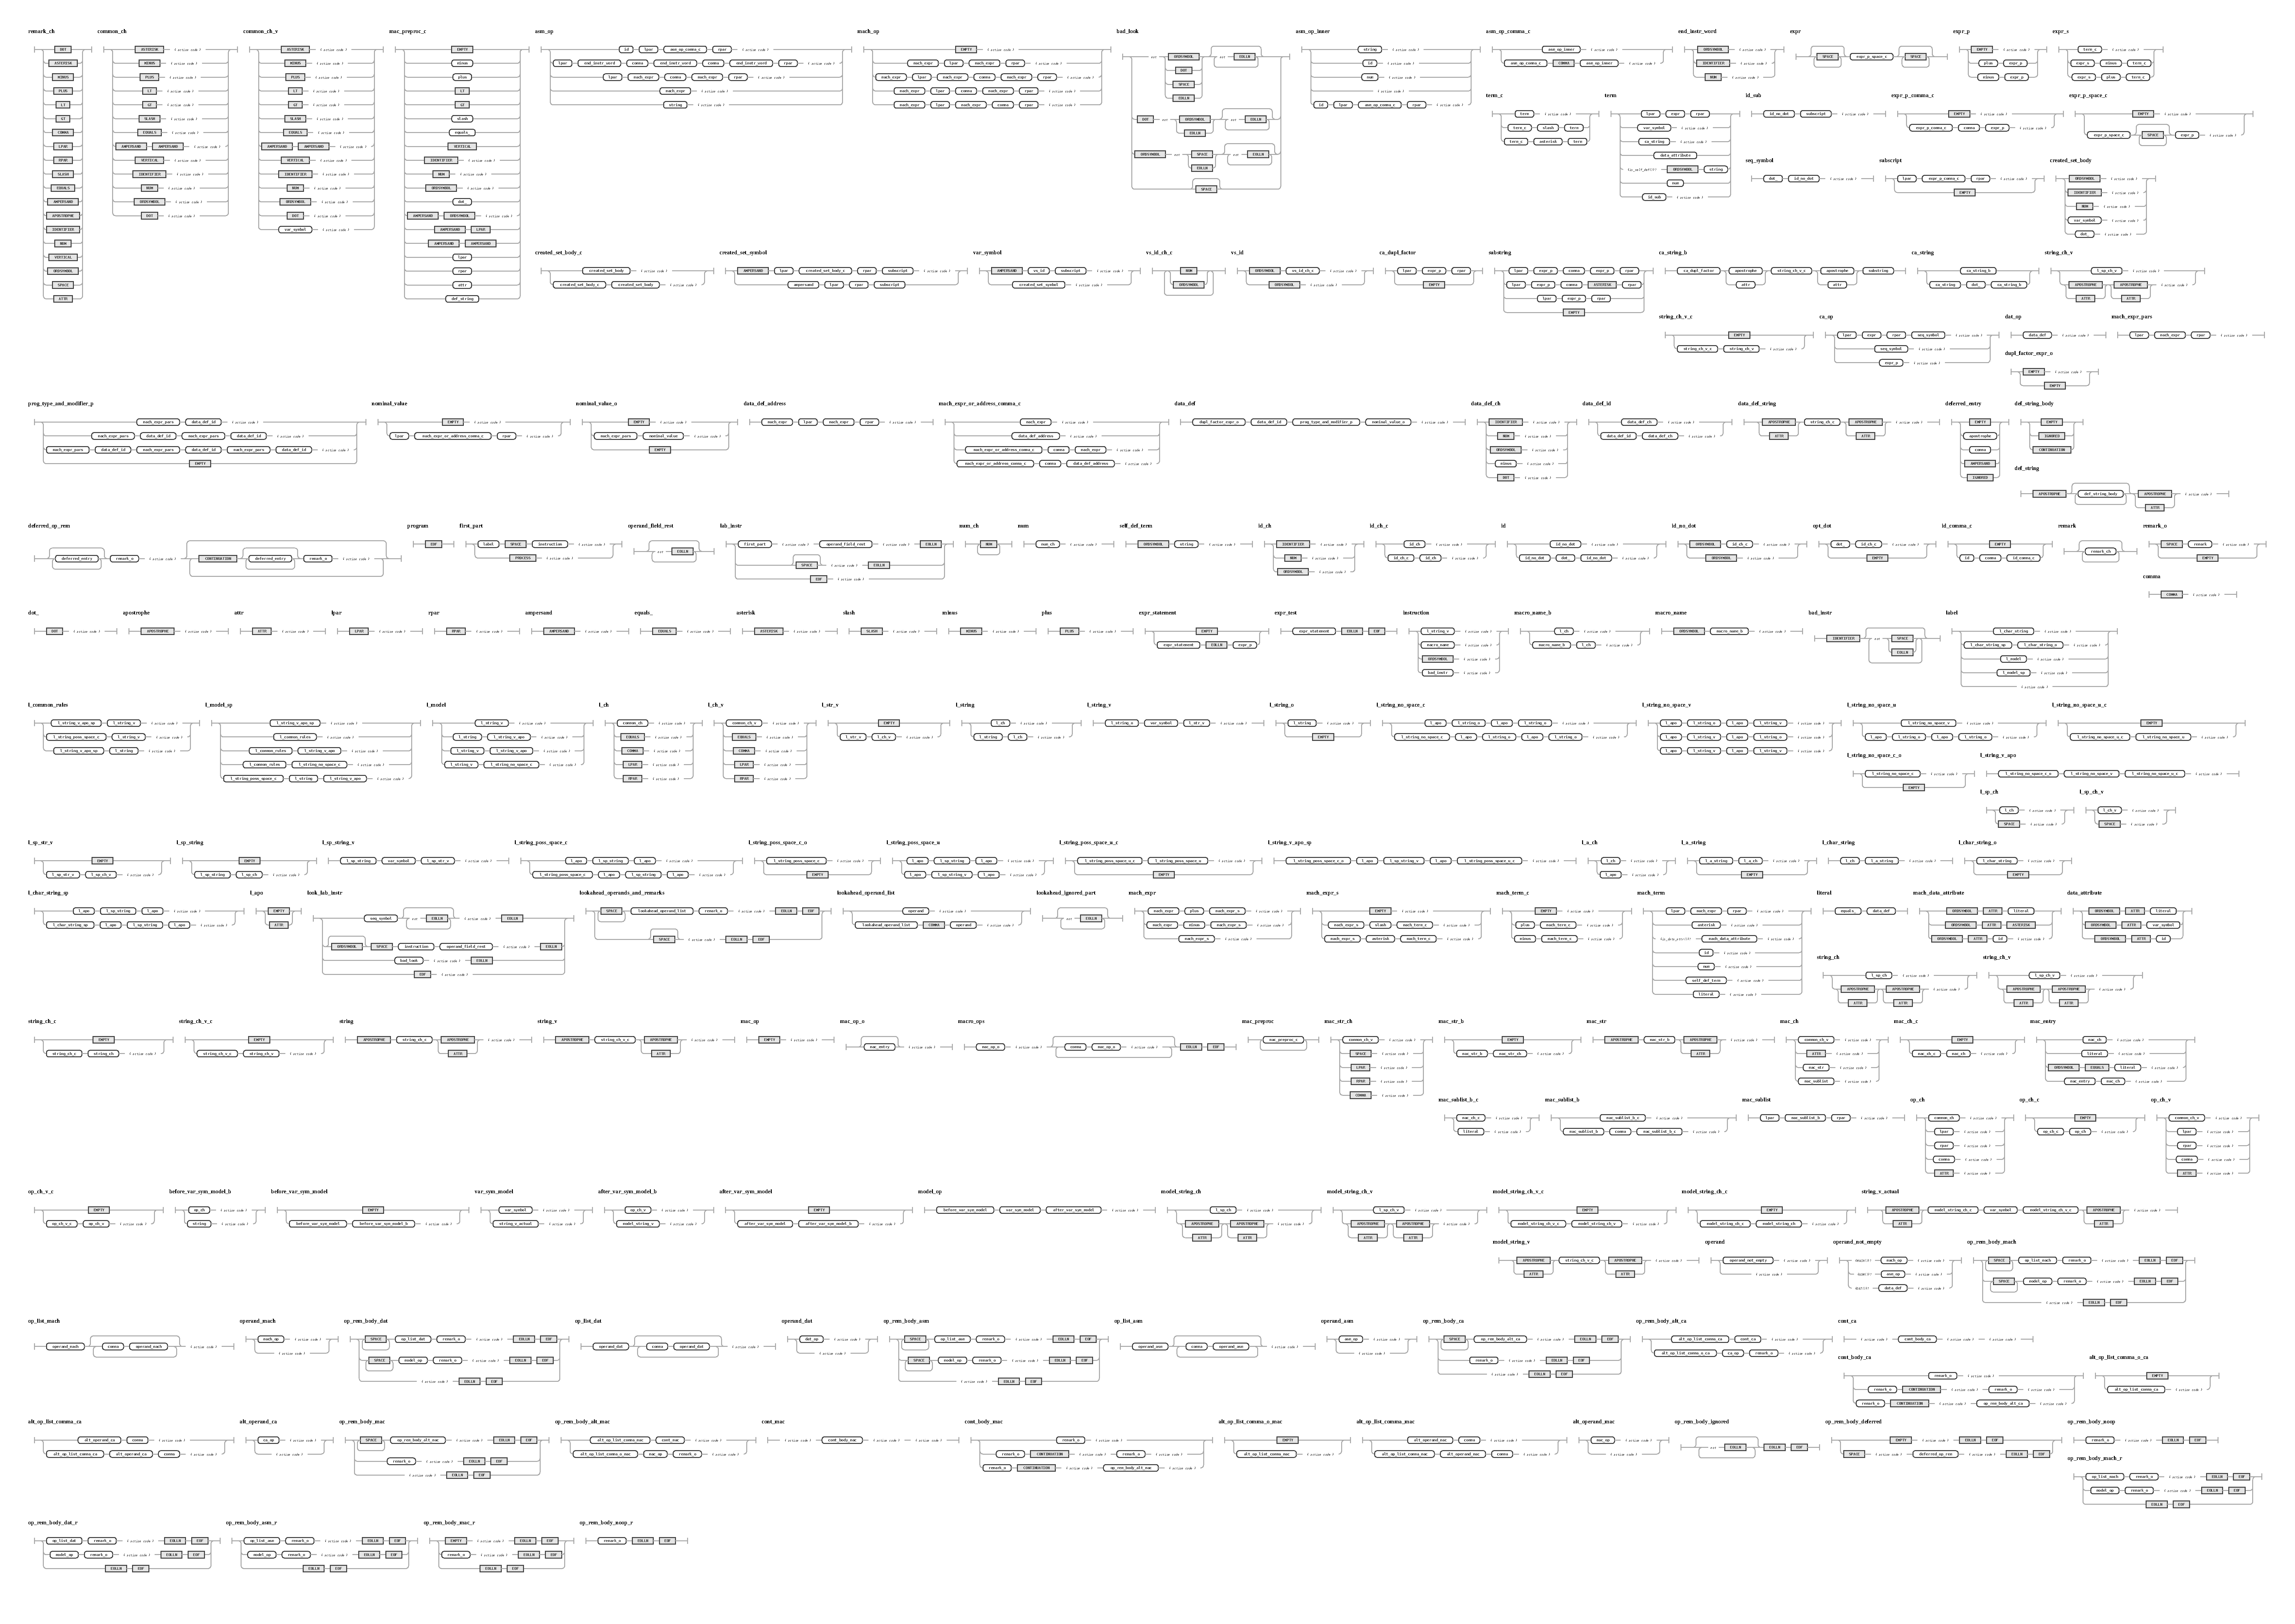
\includegraphics[width=45cm]{img/grammar}
	\caption{All 193 grammar rules}
\end{foldoutfloatlandscape}



\end{appendices}

\end{document}
